\documentclass[a4paper,12pt]{report}

\usepackage[utf8]{inputenc}
\usepackage{t1enc}
\usepackage[T1]{fontenc}
\usepackage[magyar]{babel}
\usepackage{anysize}
\usepackage[pdftex]{graphicx}
\usepackage{subfigure}
\usepackage{amsmath, amssymb, amsfonts}
\usepackage{latexsym}
\usepackage{todonotes}
\usepackage{verbatim}
\usepackage[titletoc]{appendix}
\usepackage{xcolor,listings}
\usepackage[protrusion=true,expansion=true]{microtype}
\definecolor{lightgrey}{gray}{0.95}
\lstset{
		numberstyle=\footnotesize,
		basicstyle=\ttfamily\footnotesize,
		frame=lines,
		language=Matlab,
		keywordstyle=\color{blue},
		commentstyle=\color[rgb]{0.133,0.545,0.133},
		stringstyle=\color{red},
		backgroundcolor=\color{lightgrey},
		numbers=left,
		tabsize=4,
		breaklines=true
}
%\usepackage{setspace}
%\onehalfspacing                                 % a lstlistigben \begin{singlespace*} és \end{...}, valószínűleg escape karakterek közé kellene írni, mert körülötte elrondítja
\setlength{\parindent}{0pt}
\setlength{\parskip}{1ex plus 0.5ex minus 0.2ex}
\reversemarginpar
\setlength{\marginparwidth}{2.5cm}

\newtheorem{Tet}{Tétel}[section]
\newtheorem{Lem}[Tet]{Lemma}
\newtheorem{All}[Tet]{Állítás}
\newtheorem{Kov}[Tet]{Következmény}
\newtheorem{Def}[Tet]{Definíció}
\newtheorem{Megj}[Tet]{Megjegyzés}
\newtheorem{Jel}[Tet]{Jelölés}
\newtheorem{Pl}[Tet]{Példa}
\newtheorem{Fel}[Tet]{Feladat}
\newenvironment{Mo}{\noindent \textbf{Megoldás. }}{ $\clubsuit$}
\newenvironment{Biz}{\noindent \textbf{Bizonyítás. }}{ $\square$}

\newcommand{\noun}[1]{\textsc{#1}}
\newcommand{\todored}[1]{\todo[color=red!70, size=\footnotesize]{#1}}
\newcommand{\todoor}[1]{\todo[color=orange!90, size=\footnotesize]{#1}}

\title{Szakdolgozat}

\begin{document}


% Első két oldal:



	\thispagestyle{empty}
	\begin{center}
		{\large \noun{Eötvös Loránd Tudományegyetem \\ Természettudományi Kar} }
		\line(1,0){455}
		\vspace{80pt}
		{\Huge \noun{\textbf{Véletlen iterációk statisztikai elemzése}}}
		\vspace{20pt}
		\\BSc Szakdolgozat
		\vspace{90pt}
		\\Írta: Mészáros Ádám István\\ Matematika BSc, Matematikai elemző szakirány\\
		\vspace{35pt}
		Témavezető: Sigray István\\ Műszaki Gazdasági Tanár, Analízis tanszék\\
		\vspace{100pt}
		
\includegraphics[scale=0.21]{elte.png}
		\vspace{25pt}
		\\ 2013\\ Budapest
	\end{center}
	\tableofcontents
	\setcounter{page}{1}


%%============================================================================
%%========================== szakdolgozat tartalmi része =====================
%%============================================================================

%=======================================================
%
%				0. FEJEZET
%				KÖSZÖNETNYILVÁNÍTÁS
%
%=======================================================


	\chapter*{Köszönetnyilvánítás}
		Lorem ipsum dolor sit amet, consectetur adipisicing elit, sed do eiusmod tempor incididunt ut labore et dolore magna aliqua. Ut enim ad minim veniam, quis nostrud exercitation ullamco laboris nisi ut aliquip ex ea commodo consequat. Duis aute irure dolor in reprehenderit in voluptate velit esse cillum dolore eu fugiat nulla pariatur. Excepteur sint occaecat cupidatat non proident, sunt in culpa qui officia deserunt mollit anim id est laborum.



%=======================================================
%
%				1. FEJEZET
%				BEVEZETÉS
%
%=======================================================

	\chapter{Bevezetés}
		\todoor{2013.05.14: megírtam a bevezetést}A mindennapok során gyakran szembesülünk olyan problémákkal amelyek megoldásához, vagy optimalizálásához különböző egyenleteket kell megoldanunk. Az ilyen egyenletek pontos megoldása nem mindig könnyű, vagy egyáltalán lehetséges feladat. Ilyen probléma például általános megoldóképlet hiányában az ötöd vagy magasabb fokú polinomok gyökeinek keresése. Ezen feladatok gyors megoldásánál numerikus módszerek használatára kell hagyatkoznunk.

		Ezeknek a módszereknek a gyorsaságát több tényező is kedvezőtlenül alakíthatja, így például be fogom mutatni, hogy az egyik legismertebb iterációs eljárásnál: a Newton-módszernél csak milyen esetekben garantált a konvergencia.  A dolgozatom során megpróbálok egy olyan iterációs módszert konstruálni a Newton-módszer alapján, mellyel gyors konvergenciát érthetünk el olyan helyekről is ahonnan a Newton-módszer nem, vagy csak lassan konvergál.

		A módszer konstruálásánál egy véletlen változót fogok felhasználni, amely miatt az eredmény több futtatás során több különböző eredményt is adhat. Emiatt a dolgozatom második felében ezt a módszert több példán általam írt számítógépes programokkal fogom elemezni.

		Az eredmények rekonstruálhatósága végett minden felhasznált nagyobb programot a függelékben ismertetek, és a kisebb kódokat pedig a dolgozat során kiírom és elmagyarázom.

%=======================================================
%
%				2. FEJEZET
%				A NEWTON-MÓDSZER
%
%=======================================================



	\chapter{A Newton-módszer}
    
    
    %=======================================================
    %
    %				2. FEJEZET
    %				A NEWTON-MÓDSZER
    %					|
    %					->	2.1 A módszer leírása
    %
    %=======================================================
        
        
		\section{A módszer leírása}
			A Newton-módszert, mint a neve is mutatja, először Isaac Newton dolgozta ki, azonban a mai formáját Joseph Raphson írta le 1690-ben, ezért Newton-Raphson-módszernek is hívják. Newton a módszert eredetileg polinomokra alkalmazta, ahogy a későbbiekben majd én is teszem. A Newton-módszer egy iterációs eljárás nemlineáris egyenletek gyökeinek megtalálására, közelítésére. A módszer - valós esetben - egy geometriailag nagyon egyszerű meggondoláson alapul, amit egy kép segítségével fogok bemutatni.
			
			\begin{figure}[ht]
				\centering
				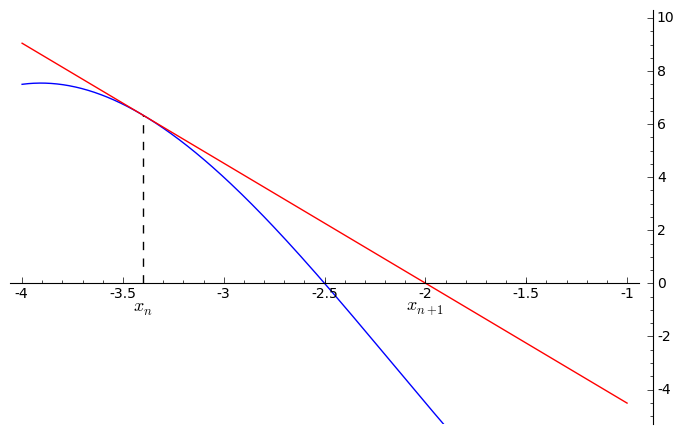
\includegraphics[scale=0.55]{kep1.png}
				\caption{Egy lépés a Newton-módszerrel}\label{k1}
			\end{figure}
			
			Első lépésként vegyünk egy kezdőpontot az $x$ tengelyen, amely elég közel van a gyökünkhöz. Jelöljük $x_0$-lal. Tegyük fel, hogy $n$ lépés után eljutottunk az $x_n$ pontig. Húzzunk érintőt a grafikonhoz ebben a pontban. Az érintő és az $x$ tengely metszéspontja legyen a következő pontunk, $x_{n+1}$, majd így folytassuk amíg elég közel nem kerülünk a egyenletünk gyökéhez. Tegyük fel, hogy $x_k$ közel van az $f(x)=0$ egyenlet $x^*$ gyökéhez, és $f$ kétszer folytonosan differenciálható. \todoor{Változtatás: következő mondat a Tanár úr megjegyzése alapján} Ekkor felírhatjuk $f$ elsőfokú Taylor-polinomját maradéktaggal a következőképpen
			\[ f(x^*)=f(x_k)+f'(x_k)(x^*-x_{k})+O((x^*-x_{k})^2) \]
			$f(x^*)$ lineáris közelítéséhez nincsen szükségünk az $(x^*-x_{k})^2$-es tagokra.
			\begin{eqnarray*}
				f(x^*)&\approx& f(x_k)+f'(x_k)(x^*-x_{k})\\
				0&\approx&\frac{f(x_k)}{f'(x_k)}+(x^*-x_{k})\\
				x^*&\approx & x_k-\frac{f(x_k)}{f'(x_k)}
			\end{eqnarray*}
			Definiáljunk egy lépést a közelítés jobb oldalával, így előállíthatjuk a következő iterációt
			\begin{equation}
				 \label{e2} x_{k+1}=x_k-\frac{f(x_k)}{f'(x_k)}
			\end{equation}
            \todoor{2013.05.14: egy plusz mondat}Amely megfelel az említett geometriai meggondolásnak.
			\begin{Pl}
				Az alábbiakban a \ref{k1}. ábrán látható polinommal fogok számolni.
				\[f(x)=x^3+6,\!5x^2+5x-12,\!5\]
				$f(x)=0$ egyenletnek gyöke az $x^*=-2,\!5$. Induljunk el az $x_0=-1$ pontból.
				\begin{center}
					\begin{tabular}{|r|r|r|r|}
						\hline
						$k$ & $x_k$     & $f(x_k)$      & $|x_k-x^*|$  \\ \hline
						$0$ & $-1,\!0000$ & $-1,\!2000e+01$ & $1,\!5000e+00$ \\ 
						$1$ & $-3,\!4000$ & $6,\!3360e+00$  & $9,\!0000e-01$ \\ 
						$2$ & $-1,\!9982$ & $-4,\!5159e+00$ & $5,\!0177e-01$ \\ 
						$3$ & $-2,\!5001$ & $8,\!6664e-04$  & $9,\!9045e-05$ \\ 
						$4$ & $-2,\!5000$ & $-9,\!8121e-09$ & $1,\!1214e-09$ \\
						\hline
					\end{tabular}
				\end{center}
			\end{Pl}
            
    	
            
    %=======================================================
    %
    %				2. FEJEZET
    %				A NEWTON-MÓDSZER
    %					|
    %					->	2.2 Konvergencia vizsgálat
    %
    %=======================================================
        
        
		\section{Konvergencia vizsgálat}
			\todoor{Változás: (2013.04.14) Kiírtam a Tanár úr által javasolt mondatokat, és átírtam a tételek feltételeit}
			Legyen $[a,b]\subset{\mathbb R}$ egy intervallum, $f:[a,b]\to {\mathbb R}$ kétszer folytonosan differenciálható és $\exists !x^*\in[a,b]$ amelyre $f(x^*)=0$. Ebben az alfejezetben azt vizsgáljuk, hogy milyen esetben tudjuk garantálni azt, hogy a Newton-módszer $f$ $x^*$ gyökéhez konvergál.
			\begin{Jel}
				\todoor{Változtatás: A jelölés részt előrébb hoztam, hogy a tételt precízebben ki tudjam mondani, és $m_1$, $M_2$ definícióit a Tanár úr megjegyzése alapján átírtam.}$m_1:=\smash{\displaystyle \min_{x \in [x_k,x^*]}} |f'(x)|$, $M_2:=\smash{\displaystyle \max_{x\in [x_k,x^*]}} |f''(x)|$, $C:=\frac{M_2}{2m_1}$
			\end{Jel}
			\begin{Tet}
			\label{t2} Tegyük fel, hogy $m_1>0$ és a Newton-módszer konvergens, ekkor másodrendben konvergál a gyökhöz.
			\end{Tet}
			\begin{Biz}
				Írjuk fel $f$ $x_k$ körüli elsőfokú Taylor-polinomját Lagrange maradéktaggal az $x^*$ pontban 
				\begin{eqnarray}
					f(x^*)&=&f(x_k)+f'(x_k)(x^*-x_{k})+\frac{f''(\xi)}{2}(x^*-x_{k})^2 \\
					0&=&\frac{f(x_k)}{f'(x_k)}+(x^*-x_{k})+\frac{\frac{f''(\xi)}{2}(x^*-x_{k})^2}{f'(x_k)}\\
					\label{e1} x^*&=&x_k-\frac{f(x_k)}{f'(x_k)}-\frac{f''(\xi)}{2f'(x_k)}(x^*-x_{k})^2
				\end{eqnarray}
				Ahol $\xi \in (x_k,x^*)$. Vonjuk ki a \ref{e2} egyenletből a \ref{e1}-est
				\begin{eqnarray*}
					x_{k+1}-x^*&=&\left(x_k-\frac{f(x_k)}{f'(x_k)}\right) - \left(x_k-\frac{f(x_k)}{f'(x_k)}-\frac{f''(\xi)}{2f'(x_k)}(x^*-x_{k})^2\right)\\
					x_{k+1}-x^*&=&\frac{f''(\xi)}{2f'(x_k)}(x^*-x_{k})^2
				\end{eqnarray*}
				\todoor{Változás: (2013.04.14) Volt egy kisebb következetlenség az abszolút értékkel}Vegyük mindkét oldal abszolút értékét
				\begin{eqnarray}
					|x_{k+1}-x^*|&=&\frac{|f''(\xi)|}{2|f'(x_k)|}|x^*-x_{k}|^2 \\
					|x_{k+1}-x^*| &\leq &C|x^*-x_k|^2 \label{e3}
				\end{eqnarray}
				Vagyis hogyha a Newton-módszer konvergens, akkor másodrendben konvergál.
			\end{Biz}

			A másodrendű konvergencia azt jelenti, hogy a hiba legalább négyzetesen csökken, vagyis a helyes jegyek száma nagyjából megduplázódik a lépésenként.
            
			Hogyan tudjuk garantálni a konvergenciát? \todoor{Változtatás: Tanár úr megjegyzése alapján a következő mondat} \ref{e3} egyenlőtlenséget a következőképpen tudjuk iterálni $x^*$ közelében
			\begin{eqnarray}
				|x_k-x^*|&\leq& C |x^*-x_{k-1}|^2\\
				&\leq & C\left |C|x^*-x_{k-2}|^2\right |^2=C^3|x^*-x_{k-2}|^4\\
				&\leq & \ldots\leq C^{2^k-1} |x^*-x_0|^{2^k}\label{e4}
			\end{eqnarray}
			Vagyis $|x_k-x^*|\leq C^{2^k-1}|x^*-x_0|^{2^k}$. Szeretnénk, ha a következő teljesülne
			\[ \lim_{k \to \infty} |x^*-x_k|=0\]
			Ha a \ref{e4} egyenletben az egyenlőtlenség jobb oldala tart nullához, akkor a Rendőr-elv alapján ez teljesül.
			\[ C^{2^k-1}|x^*-x_0|^{2^k}=q^{2^k-1}|x^*-x_0| \] 
			Ez akkor és csak akkor tart nullához, ha $q<1$.
			\[q=C|x^*-x_0|=  \frac{M_2}{2 m_1} \left |x^*-x_0 \right | < 1 \]
			Átrendezve
			\[ |x_0-x^*|<  \frac{2 m_1}{M_2} \]
			Ezek alapján a következő tételt mondhatjuk ki\todoor{Változtatás: $m_1$, $M_2$ definícióját átírtam $[a,b]$ intervallumra. Úgy gondolom így áthidaltam azt a problémát, hogy eddig ezek a konstansok függtek $x_k$-tól.}
			\begin{Tet}
				Legyen $m_1:=\min_{x \in [a,b]} |f'(x)|$, és $M_2:=\max_{x\in [a,b]} |f''(x)|$. Tegyük fel, hogy $m_1, M_2 > 0$ és $ |x_0-x^*|<  \frac{2 m_1}{M_2} $. Ekkor
				\[\smash{\displaystyle \lim_{k\to \infty} }x_k= x^*\]
			\end{Tet}
			\todoor{Változtatás: A következő eddig megjegyzés környezetben volt}Ezeket sajnos elég nehéz garantálni. Például az 5. feltételhez tudnunk kell, hogy mi a gyök, aminek a meghatározására alkalmaznánk a módszert. A 4. feltétel ellenőrzése szintén bonyolult, hiszen ehhez először meg kellene határoznunk a derivált gyökeit, amivel szintén az eredeti problémához jutunk.
			\begin{Tet}
				\label{t1}
				Tegyük fel, hogy $x_0\in [a,b]$, $\forall x \in (x^*,x_0)$-re $f'(x)$,$f''(x) \neq 0$, és $x_0$-ra teljesül, hogy $f(x_0)f''(x_0)>0$, akkor $x_k$ szigorúan monoton tart a gyökhöz.
			\end{Tet}
			\todoor{Változtatás: A tétel feltételeit átírtam hasonló stílusúra mint amiket előzőekben már használtam}
			\begin{Biz}
				Négy esetünk van.
				\begin{enumerate}
					\item $x_0>x^*$, $f(x_0)>0$
					\item $x_0>x^*$, $f(x_0)<0$
					\item $x_0<x^*$, $f(x_0)>0$
					\item $x_0<x^*$, $f(x_0)<0$
				\end{enumerate}
				Az esetek bizonyítása nagyban hasonlít, ezért csak az elsőt látjuk be. Mivel $f(x_0)>0$ és $f(x_0)f''(x_0)>0$, ezért $f''(x_0)>0$. Továbbá $(x^*,x_0)$-n $f'(x)\neq 0$, ezért az vagy mindenhol pozitív, vagy mindenhol negatív. 
				\begin{eqnarray}
					\label{e6}0&<&f(x_0)\\
					\label{e7}&=&f(x_0)-f(x^*)\\
					\label{e8}&=&f'(\xi)\underbrace{(x_0-x^*)}_{>0}
				\end{eqnarray}
				\ref{e7} $\Rightarrow$ \ref{e8} a Lagrange-féle középérték tétel miatt, valamilyen $\xi \in (x^*,x_0)$-re. Ez azt jelenti, hogy $f'(\xi)>0$, amiből következik, hogy $\forall x\in (x^*,x_0): f'(x)>0$. Ez alapján a következőt tudjuk
				\begin{eqnarray*}
					x_{k+1}&=&x_k-\underbrace{\frac{f(x_k)}{f'(x_k)}}_{>0} \\
					x_{k+1}&<&x_k
				\end{eqnarray*}
				Vagyis az $x_k$ sorozat szigorúan monoton csökkenő. Használjuk ismét a Lagrange-féle középérték tételt
				\[0<f(x_k)=f(x_k)-f(x^*)=\underbrace{f'(\xi)}_{>0}(x_k-x^*)\]
				Tehát $x_k>x^*$ azaz $x_k$ sorozat korlátos. A korlátosságból és a monotonitásból következik, hogy $x_k$ konvergens. Tegyük fel, hogy $x_k\to \tilde{x}^*$.
				\begin{eqnarray*}
					\lim_{k \to \infty} x_{k+1} &=& \lim_{k \to \infty} x_k - \dfrac{\lim\limits_{k \to \infty} f(x_k)}{\lim\limits_{k \to \infty} f'(x_k)}\\
					\tilde{x}^*&=&\tilde{x}^*-\dfrac{f(\tilde{x}^*)}{f'(\tilde{x}^*)}\\
					\dfrac{f(\tilde{x}^*)}{f'(\tilde{x}^*)}&=&0
				\end{eqnarray*}
				Ez csak akkor lehetséges, ha $f(\tilde{x}^*)=0$, viszont $x^*$ gyök egyértelmű, ezért $x^*=\tilde{x}^*$.
			\end{Biz}
            
            
    %=======================================================
    %
    %				2. FEJEZET
    %				A NEWTON-MÓDSZER
    %					|
    %					->	2.3 Leállási feltétel
    %
    %=======================================================
            
		\section{Leállási feltétel}
		\todoor{Megjegyzés: Ebben a részben nem vagyok biztos, \cite[p. 145]{na}-ben találtam az 5.2.3. tétel, de nem a Newton-módszerre szól hanem általánosan a fixpont iterációkra, de átírtam egy-két dolog, ahogy szerintem specifikus a Newton-módszerre.}  
			\begin{Jel}
				$m_1:=\smash{\displaystyle \min_{x \in (a,b)} } \left| \left( \dfrac{f(x)}{f'(x)} \right)' \right|$
			\end{Jel}
			\begin{Tet}
				Tegyük fel, hogy $f\in C^2[a,b]$ és $m_1>0$. Ekkor, ha valamilyen $\varepsilon >0 $-ra és k indexre
				\begin{equation}
					\label{e5} \left| \frac{x_{k+1}-x_k}{x_k} \right |\leq \frac{\varepsilon}{\varepsilon+1}m_1
				\end{equation}
				akkor $|x_k-x^*|\leq \varepsilon|x^*|$.
			\end{Tet}
			\begin{Biz}
				Rendezzük át a \ref{e2} egyenletet és alkalmazzuk a Lagrange-féle középérték tételt.
				\begin{eqnarray*}
					| x_{k+1} - x_{k}|&=& \left| \frac{f(x_k)}{f'(x_k)} \right| \\
					&=& \left| \frac{f(x_k)}{f'(x_k)}- \frac{f(x^*)}{f'(x^*)} \right| \\
					&=&\left| \left(\frac{f(\xi)}{f'(\xi)}\right)'\right| \cdot |x_k-x^*|
				\end{eqnarray*}
				ahol $\xi \in (x*,x_k)$
				\[| x_{k+1} - x_{k}|\geq m_1 |x_k-x^*| \]
				Fejezzük ki \ref{e5} -t $m_1$-re, és helyettesítsük be.
				\begin{eqnarray*}
					| x_{k+1} - x_{k}|&\geq& \frac{|x_{k+1}-x_k|}{|x_k|}\cdot \frac{\varepsilon+1}{\varepsilon}\cdot |x_k-x^*|\\
					\varepsilon |x_k|&\geq& \varepsilon  |x_k-x^*| + |x_k-x^*|\\
					 |x_k-x^*|&\leq &\varepsilon (|x_k|- |x_k-x^*|)\\
					&\leq& \varepsilon(|x_k-x_k+x^*|)=\varepsilon |x^*|
				\end{eqnarray*}
			\end{Biz}
			\begin{Kov}
				Tegyük fel, hogy szeretnénk $e$-nél kisebb hibával közelíteni $x^*$-ot. Mivel $|x^*|\leq\max \{ |a|,|b| \}$, ha ismerünk, egy olyan $\varepsilon$ számot, amelyre teljesül a tételbeli feltétel, és $\varepsilon \max \{|a|,|b|\} \leq e$, akkor
				\[ |x_k-x^*|\leq \varepsilon |x^*| \leq \varepsilon \max \{|a|,|b|\} \leq e \]
			\end{Kov}
			\todoor{Változtatás: Innentől kezdve minden új}
			Sajnos ez a leállási feltétel nem túl hasznos, hiszen minden lépésnél újabb $\varepsilon$-t kell keresnünk, ami műveletigényes.


    %=======================================================
    %
    %				2. FEJEZET
    %				A NEWTON-MÓDSZER
    %					|
    %					->	2.4 Komplex eset
    %
    %=======================================================


		\section{Komplex eset}
			Érdemes megvizsgálni a módszert komplex gyökkel rendelkező egyenletekre is. Ekkor a fentiekkel analóg állítások mondhatók ki. A komplex eset geometriai meggondolása is hasonló. Feleltessük meg a $z=x+yi \in \mathbb{C}$ számokat $(x,y)\in\mathbb{R}^2$ vektorokkal. Legyen $f(z)=u+vi=u(x,y)+v(x,y)i$ analitikus függvény. $|f(z)|=\sqrt{u^2(x,y)+v^2(x,y)}$. $z_k=x_k+y_ki$ ahol $f$ és $f'$ sem 0. Legyen $T_k$ $|f(z)|$ érintő síkja a $(x_k,y_k)$ helyen, és legyen $L_k$ az $xy$ sík és $T_k$ metszésvonala. Belátható, hogy ekkor \[z_{k+1}=x_{k+1}+y_{k+1}i=z_k-\frac{f(z_k)}{f'(z_k)}\] megfelel annak az $(x_{k+1},y_{k+1})$ pontnak, amelyik az $L_k$ egyenesen legközelebb van $(x_k,y_k)$ ponthoz. (\ref{k6}) \cite[p. 809]{Yau98}. A lépés iránya ezáltal ellentétes $|f(z)|$ gradiensével a $z_k$ pontban.
			
			 \begin{figure}[ht]
				\begin{center}
				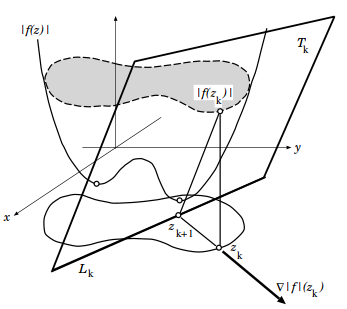
\includegraphics[scale=0.7]{kep6.png}
				\caption{A komplex eset geometriai meggondolása \cite[p. 807]{Yau98}} \label{k6}
				\end{center}
			\end{figure}
			
			Meggondolható, hogy ez valós esetben ugyanazt jelenti mint eddig, hiszen a két sík metszésvonala helyett, az $x$ tengely és $|f(x)|$ érintő egyenesének metszéspontját vesszük, ami megegyezik az $x$ tengely és $f(x)$ érintőjének metszéspontjával.

			Vegyük például a $f(x)=x^2-2i$ komplex együtthatós polinomot, amelynek az $1+i$ és a $-1-i$ a gyökei. $|f|$ gradiensénél (\ref{k7} ábra) valamivel jobb szemléltetés végett definiáljuk a következő vektormezőt
			\[g(x,y)=\left(\mathrm{Re} \left\{ -\frac{f(x+yi)}{f'(x+yi)} \right \} ,\mathrm{Im} \left\{-\frac{f(x+yi)}{f'(x+yi)}\right \} \right)\]
			Ezt ábrázolva láthatjuk, hogy az esetünkben hogyan fog haladni a komplex síkon a módszer. A \ref{k4} ábrákon jelöltem $1-0,\!5i$-ből indított módszer pontjait is. A kezdőpont pirossal van ábrázolva, ami az iterációs lépésekkel átvált sárgába.
			
			\begin{figure}[ht]
				\subfigure[$-\nabla|f(z)|$ és négy iterációs lépés az $1-0,\!5i$-ből]{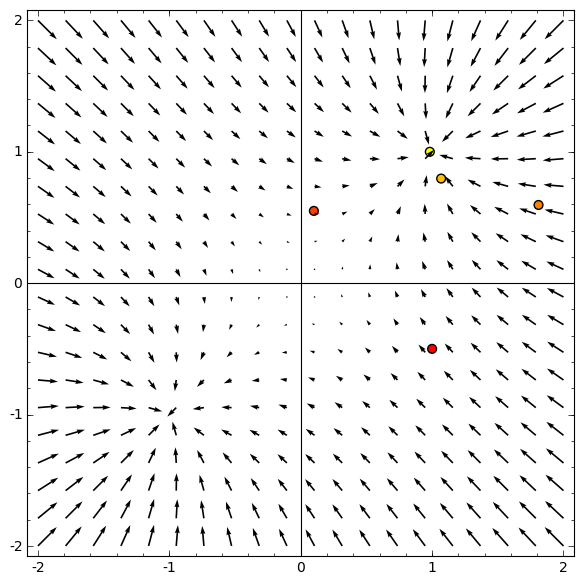
\includegraphics[scale=0.5]{kep7.png} \label{k7}}
				\hfill
				\subfigure[$g(x,y)$ és négy iterációs lépés az $1-0,\!5i$-ből]{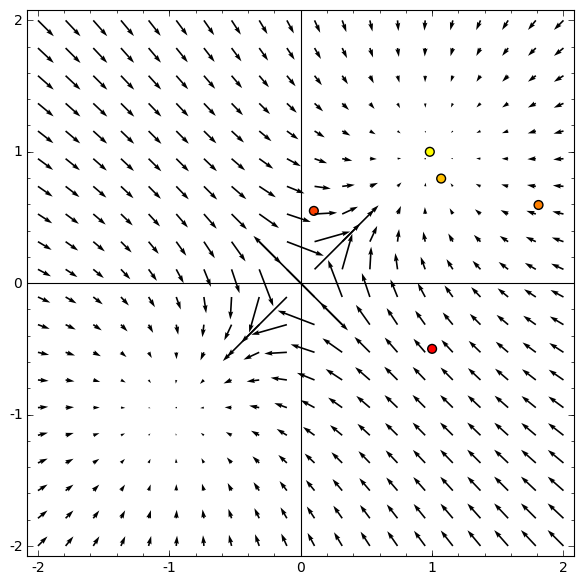
\includegraphics[scale=0.5]{kep4.png}}
				\caption{A lépés irányán túl a (b) ábra a lépés nagyságát is szemlélteti} \label{k4}
			\end{figure}
			
			\begin{Pl}
				\ref{k4} ábra számokkal, vagyis $f(x)=x^2-2i$ gyökét keressük $1-0,\!5i$ kezdőponttal.
				\begin{center}
					\begin{tabular}{|r|r|r|r|}
						\hline
						$k$ & $z_k$                & $|f(z_k)|$    & $|z_k-z^*|$  \\ \hline
						$0$ & $1,\!00000 - 0,\!50000i$ & $3,\!0923e+00$  & $1,\!5000e+00$ \\ 
						$1$ & $0,\!10000 + 0,\!55000i$ & $1,\!9125e+00$  & $1,\!0062e+00$ \\ 
						$2$ & $1,\!81000 + 0,\!59500i$ & $2,\!9261e+00$  & $9,\!0561e-01$ \\ 
						 $3$ & $1,\!06891 + 0,\!79611i$ & $5,\!8966e-01$  & $2,\!1522e-01$ \\ 
						$4$ & $0,\!98262 + 0,\!99980i$ & $4,\!8935e-02$  & $1,\!7377e-02$ \\ 
						$5$ & $1,\!00008 + 0,\!99992i$ & $3,\!0464e-04$  & $1,\!0771e-04$ \\ 
						$6$ & $1,\!00000 + 1,\!00000i$ & $1,\!1601e-08$  & $4,\!1015e-09$ \\
						\hline
					\end{tabular}
				\end{center}
			\end{Pl}
			Láthatjuk, a módszer nem csak komplex gyökökkel rendelkező valós polinomokra működik, hanem komplex együtthatós polinomokra is. Azonban ha egy valós polinom komplex gyökét szeretnénk meghatározni, akkor szükséges, hogy a kezdőpontunk képzetes része eltérjen nullától, különben az iterációs lépés tulajdonsága miatt $\forall z_k\in \mathbb{R}$ (\ref{k5} ábra).
			
			\begin{figure}[ht]
				\begin{center}
				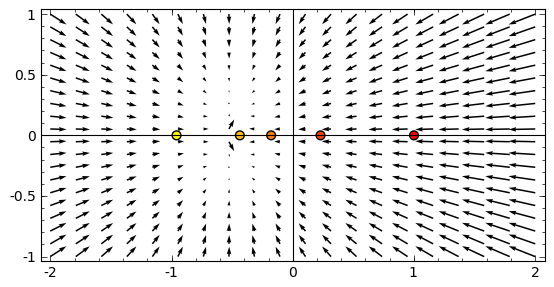
\includegraphics[scale=0.62]{kep5.png}
				\caption{$(x-( - 1/2-1/4i))\cdot (x-( - 1/2+1/4i))$ komplex gyökeinek keresése valós ($x_0=1$) kezdőpontból} \label{k5}
				\end{center}
			\end{figure}
			
			
			A komplex síkon minden gyökhöz tartozik egy vonzási tartomány, amely halmazból az iterációt indítva az adott gyökhöz konvergál a módszer. A teljes komplex síkhoz, ezenkívül hozzátartoznak azon ponthalmazok, ahonnan a módszer nem konvergens. Érdekes kérdés, hogy meg tudjuk-e határozni a gyökökhöz tartozó vonzási tartományokat adott függvényekre. A másodfokú polinomokra a következő tételt tudjuk
			\begin{Tet}[Arthur Cayley, 1897] \label{Cayley}
				Legyen $p$ komplex másodfokú polinom, melynek $\alpha$ és $\beta$ két különböző gyöke. Legyen $L$ az $\alpha$-t és $\beta$-t összekötő szakasz merőleges felezővonala. Ekkor, ha a Newton-módszert alkalmazzuk $p$-re, a gyökökhöz tartozó $B(\alpha)$ és $B(\beta)$ vonzási tartományok, az $L$ egyenes által szétválasztott komplex félsíkok.
			\end{Tet}
			Cayley nem tudta megállapítani, hogy mi teljesül nagyobb fokszámú polinomok esetén az azokon fellépő kaotikus viselkedés miatt. Ugyanis ehhez hasonló szabályos viselkedés nem figyelhető meg harmad vagy magasabb fokú polinomok esetén.
            
     
			\begin{Tet}[Gauss-Lucas]\label{GL}
				Legyen $p(z)$ egy nemkonstans komplex együtthatós polinom, $z_1,\ldots,z_n$ gyökökkel és $p'(z)$ $w_1,\ldots,w_{n-1}$ gyökökkel. Legyen $H=\{\sum_{i=1}^n c_iz_i\,\,0\leq c_i\leq 1,\,\,\sum_{i=1}^n c_i=1\}$ $p$ komplex gyökeinek konvex burka a komplex síkon. Ekkor $\forall i\,\,w_i\in H$.
			\end{Tet}
Mivel a Newton-módszer kiszámíthatatlanul viselkedik a polinom deriváltja gyökeinek a közelében, semmi biztosíték nincs arra, hogy a kezdőponthoz legközelebbi gyökhöz konvergál. Így míg a \ref{Cayley} tétel alapján erre az általánosításra számíthatnánk, a \ref{GL} tétel következményeként előfordulhat, hogy az egyik gyökhöz közel elhelyezkedő derivált gyöke, az egyik iterációs lépés során átsodorja a módszert egy másik gyökhöz közelebb. 


			Valójában minden komplex differenciálható függvényre ezen halmazok határai egy fraktált, úgynevezett Julia halmazt határoznak meg. (\ref{k10} ábra)

			\begin{figure}[ht]
				\begin{center}
				{%
					\setlength{\fboxsep}{0pt}%
					\setlength{\fboxrule}{1pt}%
					\fbox{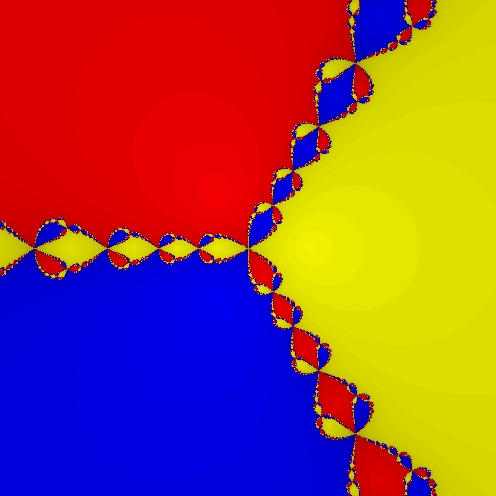
\includegraphics[scale=0.4]{fractal.png}}
				}%
				\caption{$x^3-1$ komplex gyökeihez tartozó halmazok a $\{a+bi:a,b\in[-5,5]\}$ síkrészen. A piros részből indított iteráció $-1/2+i\sqrt{3}/2$-höz konvergál, a zöld részről ennek komplex konjugáltjához, és a kék részről $1$-hez. A sötétebb részekről lassabb a módszer.} \label{k10}
				\end{center}
			\end{figure}

   			\todoor{2013.05.14: Következő rész a Tanár úr megjegyzése alapján}Ismert olyan harmadfokú polinom, amelyeknek egy adott komplex számra, és annak egy bizonyos környezetéből választott tetszőleges pontra alkalmazott Newton-módszer divergens. Az ilyen halmazokat fekete színnel szokás jelölni. Erre mutat két példát a \ref{img:div} ábra.
			\begin{figure}[ht]
				\begin{center}
				\subfigure[{Az $f(x) = (x-1)\cdot (x+0,\!5+0,\!33i) \cdot (x+0,\!5-0,\!33i)$ polinom a $\{a+bi:a,b\in[-0,\!2;0,\!2]\} $ halmazon.}]{
					\setlength{\fboxsep}{0pt}%
					\setlength{\fboxrule}{1pt}%
					\fbox{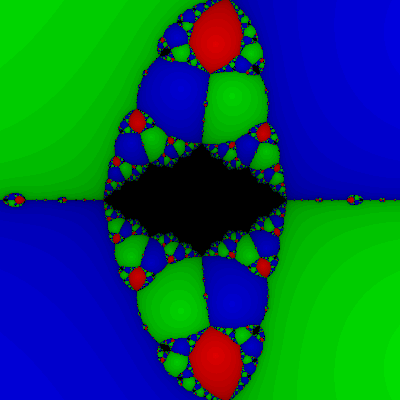
\includegraphics[scale=0.5]{frac1.png}}
				}
				\hfill
				\subfigure[{Az $f(x) = x^3-2x+2$ polinom a $\{a+bi:a,b\in[-0,\!3;0,\!3]\} $ halmazon.}]{
					\setlength{\fboxsep}{0pt}%
					\setlength{\fboxrule}{1pt}%
					\fbox{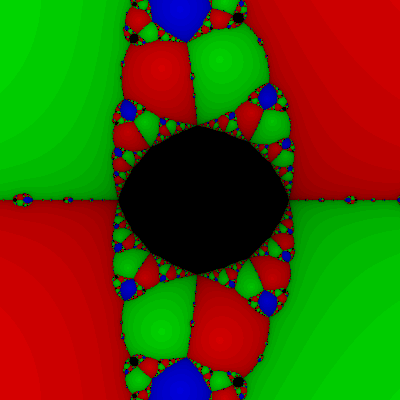
\includegraphics[scale=0.5]{frac2.png}}
				}
\caption{Példa olyan komplex halmazokra, amelyekről egy adott polinomon a Newton-módszer divergens.} \label{img:div}
				\end{center}
			\end{figure}

% poly([1   -0.5+0.33i  -0.5-0.33i])
% [1   0   -2   2]


%=======================================================
%
%				3. FEJEZET
%				MÓDOSÍTOTT MÓDSZER POLINOMOKRA
%
%=======================================================
    
    
    
\chapter{Módosított módszer polinomokra}
		Adott a Newton-módszer, amit az előző fejezetben vizsgáltunk. Tudjuk, hogyha az $x_k$ sorozat konvergens, akkor másodrendben konvergál a gyökhöz (\ref{t2}), sőt bizonyos feltételekkel monoton konvergenciát tudtunk biztosítani (\ref{t1}). Azonban sok esetben a módszer nem konvergens, ugyanis az említett tételek feltételei könnyen megsérülnek, ha a kezdőpontot nem választjuk a gyöknek egy kellően kis sugarú környezetéből. Ezt véletlenszerűen választott kezdőponttal nem tudjuk garantálni, így ilyenkor csak remélhetjük, hogy az iteráció az egyik lépés során véletlenül belelép egy megfelelő intervallumba, azzal biztosítva a további konvergenciát. Szeretnénk egy olyan módszert, amely ennek ellenére konvergens viszonylag gyorsan és sok helyről.\todoor{Változás: (2013.04.14) Megpróbáltam saját szavaimmal belefűzni amit a Tanár úr javasolt. Az eredeti szöveg a kódban kommentben még megtalálható.}
		 \begin{comment}
			A sz\"ovegbe menjen: A probl\'ema ugyanis az, hogy a konvergenciavizsg\'alataink csak lok\'alisak voltak, azaz csak akkor garant\'alt\'ak a konvergenci\'at, amikor a gy\"okh\"oz kell\H oen k\"ozelr\H ol indultunk. Ez term\'eszetesen nem teljes\"ul egy v\'eletlen\"ul v\'alasztott  kezd\H opont eset\'en. Ilyen esetben csak abban lehet rem\'enykedni, hogy az iter\'aci\'o "v\'eletlens\'egb\H ol" egyik l\'ep\'es sor\'an k\"ozel ker\"ul a gy\"okh\"oz. 
        
			Ennek a k\'erd\'esnek nagy elm\'elete van, \'es paradox m\'odon a komplex esetben lehet t\"obbet tudni, mint a val\'os esetben.
		\end{comment}

    %=======================================================
    %
    %				3. FEJEZET
    %				MÓDOSÍTOTT MÓDSZER POLINOMOKRA
    %					|
    %					->	3.1 Motiváció
    %
    %=======================================================


		\section{Motiváció}
			Vizsgáljuk meg, hogy egy polinom hogyan viselkedik a \ref{t1} tétel alapján, vagyis honnan indulva garantált a monoton konvergencia.
			
			\begin{figure}[ht]
				\centering
				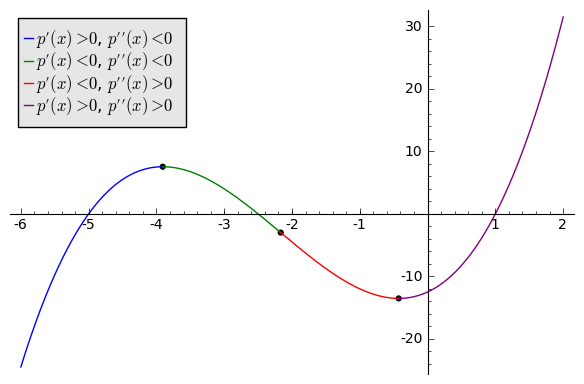
\includegraphics[scale=0.6]{kep2.png}
				\caption{Egy polinom felosztása az első és második deriváltjának viselkedése alapján}\label{k2}
			\end{figure}
			
			A tétel feltételei alapján a kezdőpontunk és a gyök közötti intervallumon sem a függvény deriváltja, sem a második deriváltja nem lehet nulla. Ez négy lehetőséget ad melyet a \ref{k2} ábrán szemléltettem. Mint az ábrán is látható, előfordulhat olyan eset, amikor egy ilyen intervallumon nincsen gyöke a polinomnak. Azonban amelyik intervallumon van, ott a gyök előtti, vagy utáni részről véve a kezdőpontunkat a feltételek teljesülnek.
			
			\begin{figure}[ht]
				\centering
				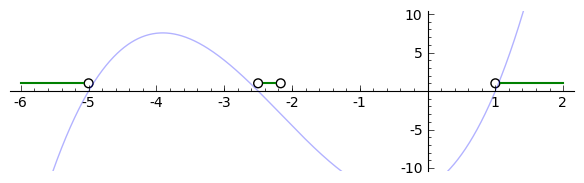
\includegraphics[scale=0.6]{kep3.png}
				\caption{Megfelelő intervallumok a kezdőpont választáshoz \ref{t1} tétel alapján}\label{k3}
			\end{figure}
			
			Láthatjuk, hogy esetünkben a kezdőpontunknak alkalmas intervallum majdnem lefedi a számegyenest, \todoor{Változás: (2013.04.14) töröltem egy mondatot ami tartalmilag már nem tetszett nekem}és bár monoton és másodrendű konvergencia garantált, a két szélső intervallumban, ha távolról indulunk előfordulhat, hogy lassú lesz a módszer.

			Ha egy polinomot leosztunk egy másik polinommal, és a két polinomnak nem egyezik meg valamelyik gyöke, akkor egy olyan függvényt kapunk amelynek a gyökei megegyeznek az eredeti polinoméval. Ugyanis legyen $p_1(x)$ a polinomunk amelyiknek a gyökeit keressük, és osszuk le $p_2(x)$ polinommal. Legyen $x^*$ gyöke $p_1(x)$-nek. Ekkor
			\[ \frac{p_1(x^*)}{p_2(x^*)}=\frac{0}{p_2(x^*)}=0\]
			Felvetődik tehát az ötlet, hogy hajtsuk végre a Newton-módszert a $\frac{p_1(x)}{p_2(x)}$ egyenlet gyökeinek keresésére. Vegyük azt a speciális esetet, amikor $p_2(x)=p_1'(x)$. Ha $p_1(x)$-nek nincs többszörös gyöke, akkor a módosított egyenletünknek ugyanazok a gyökei.
			
			\begin{figure}[ht]
				\subfigure[Egy polinom és a módosított egyenlete]{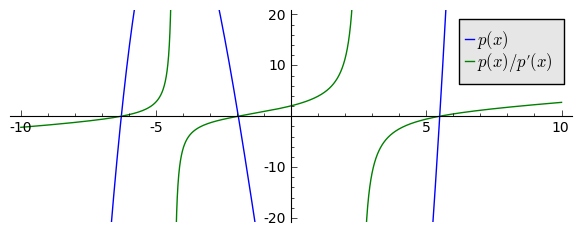
\includegraphics[scale=0.5]{sage8.png} \label{k8}}
				\hfill
				\subfigure[Megfelelő intervallumok a kezdőpont választáshoz \ref{t1} tétel alapján]{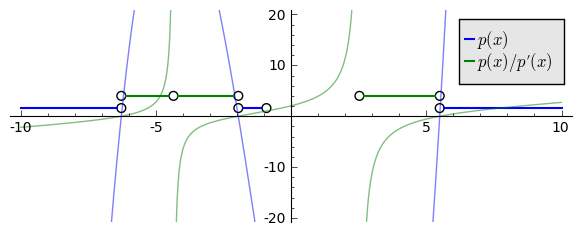
\includegraphics[scale=0.5]{sage9.png} \label{k9}}
				\caption{}
			\end{figure}
   


    %=======================================================
    %
    %				3. FEJEZET
    %				MÓDOSÍTOTT MÓDSZER POLINOMOKRA
    %					|
    %					->	3.2 A módszer
    %
    %=======================================================


		\section{A módszer}
            
			Ahogyan a \ref{k9} ábrán látható a két egyenlet konvergenciát garantáló intervallumai jól kiegészítik egymást. Ez alapján az az ötletünk támadhat, hogyha véletlenszerűen váltogatjuk az egyenletet, amire a módszert alkalmazzuk, jó eséllyel eljutunk az egyenletünk valamelyik gyökéhez.

			Tehát adott $p$ polinom, amelynek a gyökeit keressük. Ekkor vegyük azt az iterációt, aminek egy lépését $0,\!5$ valószínűséggel a (\ref{e9}) iterációval tesszük, és $0,\!5$ valószínűséggel (\ref{e10}) iterációval. 
			\begin{eqnarray}
				\label{e9}x_{k+1}&=&x_k- \frac{p(x_k)}{p'(x_k)}\\
				\label{e10}x_{k+1}&=&x_k-\frac{\frac{p(x_k)}{p'(x_k)}}{\left(\frac{p(x_k)}{p'(x_k)}\right)'}=x_k-\frac{p(x_k)p'(x_k)}{p'(x_k)^2-p''(x_k)p(x_k)}
			\end{eqnarray}
			A későbbiekben ezekre első (\ref{e9}), és második (\ref{e10}) iterációs lépésként fogok hivatkozni.
			\begin{Pl}
				Az alábbiakban egy olyan harmadfokú polinomon végzem el az iterációt, aminek az együtthatóit $-50$ és $50$ között véletlenszerűen generáltam.
				\[f(x)=-49,\!6776x^3+36,\!1231x^2-1,\!1662x-20,\!4780\]
				\begin{center}
					\begin{tabular}{|r|r|r|r|r|}
						\hline
						$k$ &   iterációs lépés &   $x_k$                   &   $|f(x_k)|$      &   $|x_k-x^*|$  \\ \hline
						$0$ &   -               &   $1+i$                   &   $8.2695e+01$    &   $5.5794e-01$ \\ 
						$1$ &   1.              &   $0,\!78752 + 0,\!72275i$    &   $2,\!0696e+01$    &   $2,\!0946e-01$ \\ 
						$2$ &   2.              &   $0,\!60295 + 0,\!54236i$    &   $3,\!4869e+00$    &   $4,\!9152e-02$ \\ 
						$3$ &   1.              &   $0,\!64583 + 0,\!57250i$    &   $2,\!7337e-01$    &   $3,\!6089e-03$ \\ 
						$4$ &   2.              &   $0,\!64227 + 0,\!57184i$    &   $1,\!3524e-03$    &   $1,\!7911e-05$ \\ 
						$5$ &   1.              &   $0,\!64228 + 0,\!57183i$    &   $3,\!3361e-08$    &   $4,\!4183e-10$ \\
						\hline
					\end{tabular}
				\end{center}
			\end{Pl}
			\begin{Pl}
				Egy szemléletesebb példaként hajtsuk végre a módszert a következő polinomon $x_0=5$ kezdőponttal
				\[p(x)=x^3+2x^2-5x-6\]
				
				\begin{figure}[ht]
					\centering
					\subfigure[Az első iterációs lépéssel lépünk]{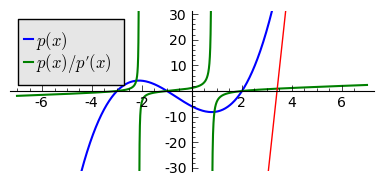
\includegraphics[scale=0.71]{0.png}}
					\hspace{3mm} % két kép közötti távolság
					\subfigure[Az első iterációs lépéssel lépünk]{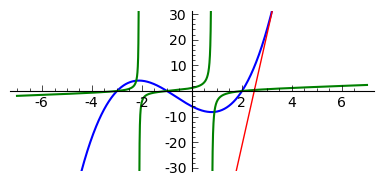
\includegraphics[scale=0.71]{1.png}}\\
					\subfigure[Az második iterációs lépéssel lépünk]{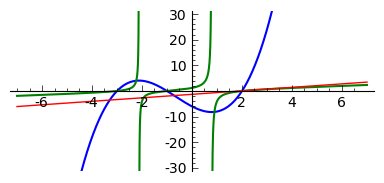
\includegraphics[scale=0.71]{2.png}}
					\hspace{3mm} % két kép közötti távolság
					\subfigure[Az első iterációs lépéssel lépünk]{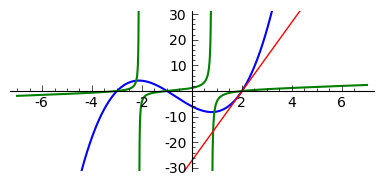
\includegraphics[scale=0.71]{3.png}}
				\end{figure}
				
				Az ábrán a következő lépések láthatók: $x_1=3,\!4$, $x_2=2,\!4891$, $x_3=1,\!9040$, $x_4=2,\!0053$. Megfigyelhető az ábrákon, hogy a negyedik lépéssel elég közel kerültünk a gyökhöz, az ábrákat továbbfolytatni ezáltal fölösleges helyfoglalás lenne, viszont a következő lépés megtalálja az $x^*=2$ gyököt. (\ref{pontossag} megjegyzés)
			\end{Pl}




    %=======================================================
    %
    %				3. FEJEZET
    %				MÓDOSÍTOTT MÓDSZER POLINOMOKRA
    %					|
    %					->	3.3 Elemzés
    %
    %=======================================================

			\section{Elemzés}
				\todoor{Megjegyzés: (2013.04.17) Elég nehezen tudtam elkezdeni ezt a részt, úgyhogy úgy döntöttem egyelőre leírok minden gondolatot amit tudok az új módszerről, és a később majd a Tanár úr segítségével meglátjuk, hogy mi az amire szükség van a dolgozatban, vagy milyen irányba kellene inkább indulnom}A dolgozat következő szakaszában az imént bevezetett módszert fogjuk több szempontból megvizsgálni. A vizsgálathoz több helyen a GNU Octave programnyelvet használom, ami szinte teljesen kompatibilis a MATLAB-bal, emellett ingyenes. A programok bemutatására ebben a fejezetben nem szánok sokat, csak éppen annyit, hogy érthető legyen az elvégzett művelet. A programok részletesebb bemutatását bővebben az \ref{Appendix} függelékben végzem.
				\todoor{2013.05.12. változás: A következő megjegyzés a számítások hibájáról, a Tanár úr megjegyzése miatt}
				 \begin{Megj}\label{pontossag}Szükségesnek tartom megjegyezni a programokkal számolt közelítések hibájának mértékét. Minden program a  \texttt{Newton.m} programot használja fel a Newton-módszer elvégzéséhez. Ennek a felhasználó az 5. argumentumában be tud állítani egy hibakorlátot, amelyet ha nem adunk meg akkor a $0,\!001$ alapbeállítással dolgozik. A programokban is végig ezt az értéket használtuk. A hibakorlát a relatív közelítési hibát korlátozza vagyis akkor mondjuk, hogy megtalálta a gyököt, ha\[\frac{|x_i-x_{i-1}|}{|x_i|}<0,\!001.\]
				\end{Megj}
				Egy iterációs eljárás vizsgálatakor elsősorban az érdekelhet minket, hogy konvergens-e a módszer, és ha igen, akkor milyen gyorsan konvergál. Ezek megvizsgálásához egy olyan módszernél, amelyben egy véletlen változó befolyásolja az eredményt, a statisztika módszereire lesz szükségünk.
				\begin{All}
					Tegyük fel, hogy $p$ polinomra és egy adott $x^*$ gyökére teljesülnek a \ref{t2} feltételei, $p$-nek $x^*$ nem többszörös gyöke, és $p''(x)p(x)\neq p'(x)^2$. Ekkor \ref{e10} másodrendben konvergál a gyökhöz.
				\end{All}
				\begin{Biz}
				    A második iterációs lépés nem más, mint a Newton-módszer a $p/p'$ egyenletre, aminek adott gyöke megegyezik $p$ gyökével, így ha $p/p'$-re teljesülnek \ref{t2} feltételei, akkor mivel $p/p'$ adott gyökéhez másodrendben konvergál, így $p$ gyökéhez is. $p/p'$ folytonos azon a helyen kívül, ahol $p'=0$. Ezáltal kiválaszthatók a megfelelő $[a,b]$ intervallumok a gyökök körül, amely nem tartalmazzák $p'$ gyökhelyeit. 
				    
				    $m_1>0$-hoz azt kell belátnunk, hogy $(p/p')'\neq 0$
				    \[\left( \frac{p(x)}{p'(x)} \right)'=1-\frac{p''(x)p(x)}{p'(x)^2}\]
				    Tehát amennyiben $p''(x)p(x)=p'(x)^2$ teljesül valamilyen $x$-re, ott a függvényünk deriváltja $0$. Ezért tettük fel, hogy ez nem teljesül. Ehhez létezik megfelelő $[a,b]$ intervallum, hiszen ahol $p/p'=0$ ott a derivált $1$.
				    
				    $p/p'$ kétszer folytonosan differenciálható, ugyanis
				    \[\left( \frac{p(x)}{p'(x)} \right)''=\left(1-\frac{p''(x)p(x)}{p'(x)^2}\right)'=-\frac{p'''(x)p'(x)^2p(x)+p''(x)p'(x)^3-2p''(x)^2p'(x)p(x)}{p'(x)^4}\]
				    A számlálóban végzett folytonos függvények közötti műveletek nem befolyásolják a függvény folytonosságát, így az csak ott nem folytonos, ahol $p'(x)=0$, vagyis $p/p'$ $[a,b]$-n kétszer folytonosan differenciálható.
				\end{Biz}
				
				Tehát ha megfelelő a polinomunk akkor (a megfelelő helyeken) két másodrendű módszert használunk véletlenszerűen váltakozva.

				\todoor{2013.05.14: Beszúrtam egy kis megjegyzést}Azonban ha a polinomnak van többszörös gyöke, akkor sem kizárt, hogy a második iterációs lépés megtalálja a gyököt. Vegyük például a $p(x)=x(x-3)^2$ polinomot melynek a $3$ kétszeres gyöke. 

				\begin{figure}[ht]
					\centering
					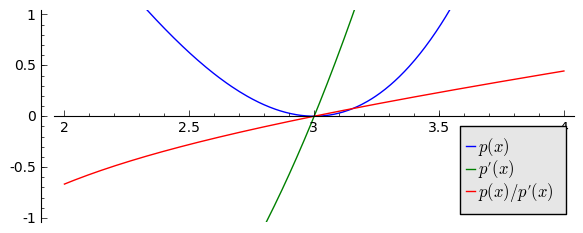
\includegraphics[scale=0.7]{multi.png}
					\caption{$p(x)=x(x-3)^2$ polinom, annak deriváltja és a hányadosuk ábrázolása.}\label{img:multiple}
				\end{figure}

			
			\ref{img:multiple} ábrán látható, hogy bár $p'(x)$-nek is gyöke a $3$, annak környezetében abszolút értékben nagyobb értékeket vesz fel mint $p(x)$, ami miatt a hányados bár nem értelmezett $3$-ban, de \[\lim_{x\to3}\frac{p(x)}{p'(x)}=0\]
				Ez nekünk annyira pont elég, hogy a módszer, ahogyan közeledik $3$-hoz úgy egy idő után megálljon a hibahatár elérésekor.

				Statisztikai elemzéshez különböző adatok generálására lesz szükségünk. Ezelőtt vizsgáljuk meg a módszerek konvergenciáját és annak idejét egy-két példában, amiből későbbiekben intuitív ki tudunk indulni. Érdemes lenne olyan példákat találni amelyeken működik a módszer és olyanokat is amelyeken nem, ezáltal össze tudnánk vetni, hogy mi befolyásolhatja a módszer helyességét.
				\subsection{Egy példán keresztül}
				Vegyünk egy harmadfokú polinomot és vegyünk olyan kezdőpontot amely elég távol van a gyöktől.
				\begin{lstlisting}[caption=Bemenet]
p=poly([1,6+3i,6-3i])
[gyok,it]=Newton(p,2e+4)
				\end{lstlisting}
				Az első sorban létrehozom a $p$ polinomot melynek három gyöke $1$, $6+3i$ és $6-3i$. A második sorban egy saját függvényt használok fel (\ref{Newton}), amely a $p$ polinomon végzi el a Newton-módszert $x_0=20000$ kezdőponttal.
				\begin{lstlisting}[caption=Eredmény]
gyok =  1.00000
it =  29
				\end{lstlisting}
				Vagyis a Newton-módszer 29 lépés alatt találta meg az $x^*=1$ gyököt. Nézzük a Newton-módszert $p/p'$ egyenleten!
				\begin{lstlisting}[caption=Bemenet]
[gyok,it]=Newton(p,2e+4,0,2)
				\end{lstlisting}
				\begin{lstlisting}[caption=Eredmény]
gyok =  1.0000
it =  9
				\end{lstlisting}
				Vagyis a módosított egyenletünkkön végrehajtott módszer gyorsabban találta meg ugyanazt a gyököt. Nézzük a véletlen iterációt!
				\begin{lstlisting}[caption=Bemenet,escapeinside={@}{@},label={lst:first}]
x=zeros(1e+4,1);
for i=1:(1e+4)
	[gyok,it]=Newton(p,2e+4,0,3);
	x(i)=it;
end
m=mean(x)
s=std(x)
figure('Position',[10 10 450 300])
hax=axes;
hold on
@\label{lst:hist}@hist(x)
line([29 29],get(hax,'YLim'),'Color',[1 0 0]) % Szukseges lepesszam p-n
line([9 9],get(hax,'YLim'),'Color',[0 0 1]) % Szukseges lepesszam p/p'-n
				\end{lstlisting}
				Elvégzem $10000$-szer a módosított módszert ugyanazon bemenő paraméterekkel, majd kiszámolom a szükséges lépések számának átlagát és szórását, ezenkívül egy hisztogramon is ábrázolom, hogy lássuk az eloszlását (\ref{k11} ábra).
				\begin{lstlisting}[caption=Eredmény]
m =  14.298
s =  4.9452
				\end{lstlisting}
				
				\begin{figure}[ht]
					\centering
					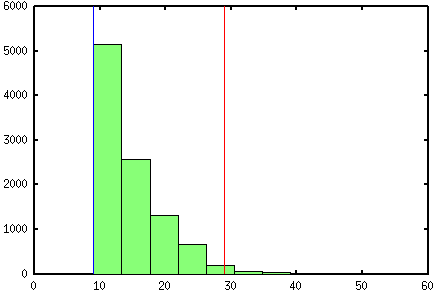
\includegraphics[scale=0.65]{hist.png}
					\caption{\ref{lst:first} listázás \ref{lst:hist}. sorának eredménye, amely szemlélteti a véletlen iterációhoz szüksges lépések számának eloszlását, az adott esetben. A piros vonal a Newton-módszer szükséges lépésszámát jelzi $p$-n, a kék vonal $p/p'$-n}\label{k11}
				\end{figure}
				
A lépések száma átlagosan megfeleződött, ami egyelőre jó eredménynek tűnik, bár megjegyzem, hogy nem vizsgáltam, hogy minden futtatás elérte-e egy gyököt. Ami a hisztogramról elsőre feltűnik, hogy nagyobb a valószínűsége, hogy hamar véget ér az iteráció, és egyszer sem volt gyorsabb mint a két iterációs lépésből a gyorsabb külön futtatva, viszont előfordult, hogy lassabb mint a lassabb iteráció. Persze ebből még ne vonjunk le semmit. Futtassuk le a fenti kódokat egy távoli komplex kezdőponttal: $x_0=20000-10000i$
				\begin{lstlisting}[caption=Eredmény]
gyok =  6.0000 - 3.0000i
it =  26
m =  14.319
s =  4.9417
				\end{lstlisting}
				Az első két sor a Newton-módszer eredménye, a harmadik, negyedik a véletlen iterációé. Az előzőtől lényeges különbséget egyelőre nem látunk, érdemes lenne sokkal több pontot egyszerre vizsgálni. 

				Nézzük meg a véletlen iteráció milyen eloszlásban iterált a gyökökhöz. 
				\begin{lstlisting}[caption=Bemenet]
r=roots(p); % [6.0000 + 3.0000i,6.0000 - 3.0000i,1.0000 + 0.0000i]
n=length(r)+1;
y=zeros(1,n);
for j=1:(1e+4)
	[gyok,it]=Newton(p,1e+4*(2-i),0,3);
	[MINE,MINH]=min(abs(r-gyok));
	if MINE<0.001
		y(MINH)=y(MINH)+1;
	else
		y(n)=y(n)+1;
	end
end
y/1e+4 % vagy abrzolashoz: x=1:n; bar(x,y/1e+4);
				\end{lstlisting} 
				A GNU Octave beépített függvényével kiszámolom a polinom gyökeit (ami egyébként a Frobenius kísérő mátrix sajátértékeivel határozza meg őket), majd elvégzem 10000-szer a véletlen iterációt, és eltárolom melyik esetben melyik gyökhöz konvergált a módszer. Végül pedig kiszámolom a relatív gyakoriságokat.
				\begin{lstlisting}[caption= Eredm\'eny]
ans =

   0   0   1   0
				\end{lstlisting} 
                Az eredmény szerint a módszer 1 valószínűséggel tart a 3. gyökhöz, ami az $1+0i$. Ez azt jelenti, hogy az előzőekben kapott eredményeknél, de legalábbis a komplex kezdőpontnál, a véletlen iteráció mindig elérte a gyököt, ami ráadásul nem egyezik meg a Newton-módszer által megtalált gyökkel. A 4. elem annak a relatív gyakorisága, hogy nem konvergál a módszer. 

				Az előző példákra egy általánosabb módszert is felépíthetünk, amely egy polinomnál egyszerre több pontból is megvizsgálja, hogy konvergál-e a módszer és átlagosan milyen gyorsan. Továbbá érdekes lehet a véletlen iteráció és az eredeti módszerek konvergencia sebességének összefüggése, mint minden véletlen iteráció konvergencia sebessége lassabb mint valamelyik módszeré, vagy van-e esély arra, hogy ahonnan semelyik módszer nem konvergált, ott a véletlen iteráció igen.
				
				A következőkben a \ref{Konvergencia} függelékben ismertetett függvénnyel szemléltetem az adott polinomon a véletlen iteráció jóságát.
				\begin{lstlisting}[caption=Bemenet,escapeinside={@}{@},label={lst:piter}]
@\label{lst:piter1}@IteracioAbraKomplex(p,-20-25i,30+25i,100,1,1)
@\label{lst:piter2}@IteracioAbraKomplex(p,-20-25i,30+25i,100,1,2)
@\label{lst:piter3}@IteracioAbraKomplex(p,-20-25i,30+25i,100,100,3)
				\end{lstlisting}
				A hívott program az adott polinomhoz készít egy szemléltető ábrát a $\{a+bi:a\in[-20,30],\,b\in[-25,25]\}$ komplex számhalmazon az adott módszerekhez. Bár ez a halmaz nem tartalmaz a gyöktől távoli számokat, mégis érdekesebbnek tűnt ezen összehasonlítást végezni. Az első ábra a sikeresen gyökhöz ért iterációk számát szemlélteti. Ez az első két esetben 0 vagy 1, így csak az utolsó esetben érdekes, ahol a véletlen változó miatt előfordulhat, hogy egy pontból egyszer konvergens a módszer, egyszer nem, itt 100 ismétlést végzünk. A második ábra a sikeres esetekhez szükséges iterációs lépések számát mutatja. A listázás három sorával mindkét ábrát kirajzoljuk mindegyik módszerhez $100\cdot 100$ kezdőpontból indulva.
				
				\begin{figure}[ht]
					\centering
					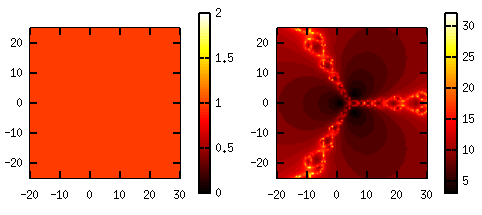
\includegraphics[scale=0.7]{p-iter1.png}
					\caption{\ref{lst:piter} listázás \ref{lst:piter1}. sorának eredménye, amely szemlélteti a Newton-módszer konvergenciáját az adott polinomon, és az ahhoz szükséges lépések számát. A módszer mind a $100\cdot 100$ kezdőpontból konvergens volt} \label{fig:piter1}
				\end{figure}
				
				\begin{figure}[ht]
					\centering
					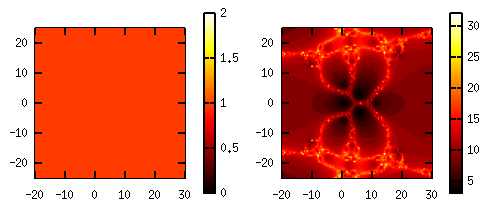
\includegraphics[scale=0.7]{p-iter2.png}
					\caption{\ref{lst:piter} listázás \ref{lst:piter2}. sorának eredménye, amely szemlélteti a Newton-módszer konvergenciáját a $p/p'$ egyenleten, és az ahhoz szükséges lépések számát. A módszer mind a $100\cdot 100$ kezdőpontból konvergens volt.} \label{fig:piter2}
				\end{figure}
				
				Láthatjuk, hogy a különböző egyenletekre futtatott Newton-módszer (\ref{fig:piter1} ábra és \ref{fig:piter2} ábra) máshol éri el a kritikusabb, lassabb pontjait. Amik a gyökök vonzási tartományának határain helyezkednek el.
				
				\begin{figure}[ht]
					\centering
					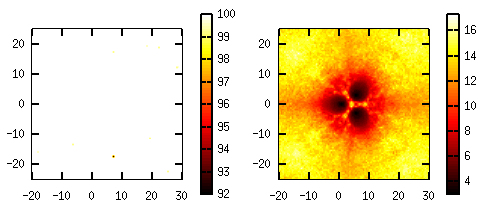
\includegraphics[scale=0.7]{p-iter3.png}
					\caption{\ref{lst:piter} listázás \ref{lst:piter3}. sorának eredménye, amely szemlélteti a véletlen iteráció konvergenciáját az adott polinomon, és az ahhoz szükséges lépések átlagos számát. A módszer $100\cdot 100$ kezdőpontból indulva pár pontból nem konvergált minden esetben, de a legrosszabb esetben is $0,\!92$ valószínűséggel igen. Cserébe a leglassabb esetben is átlagosan $17$ lépés alatt megtalált egy gyököt.} \label{fig:piter3}
				\end{figure}
				
				Bár előfordulhat, hogy a képek alapján nem megfelelő következtetéseket vonunk le, érdemes szemügyre venni az eredményeket mielőtt az adatokkal foglalkoznánk. Ami feltűnő, hogy a véletlen iterációnak a leglassabb esetében is átlagosan csak 17 iterációs lépésre volt szüksége, míg a különböző egyenletekre külön néhol 30 fölé emelkedik ez a szám. Ha a felosztást finomítjuk az ábrákon látható tendencia mentén megtalálna olyan kezdőpontokat, ahonnan lassabb az iteráció, míg a véletlen iteráció esetén a máshol elhelyezkedő kritikus kezdőpontok miatt a szükséges lépések száma, meglátásom szerint, nem fog lényegesen megnőni. Viszont megfigyelhető, hogy a \ref{fig:piter1} és \ref{fig:piter2} ábráktól eltérően itt az ábra nagy része világos, vagyis a pontok nagy részénél szükség is volt 13-17 lépésre, míg a különálló módszereknél a 10 lépéshez tartozó árnyalatok dominálnak.

				\ref{app:megj} megjegyzés alapján rajzoljuk ki a véletlen iterációhoz szükséges lépések számának minimumát és maximumát. (\ref{img:megj} ábra)
				
				\begin{figure}[ht]
					\centering
					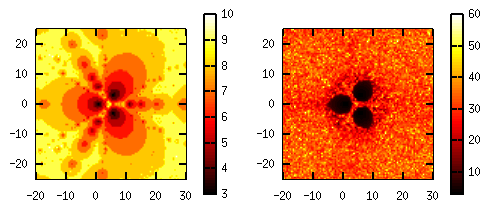
\includegraphics[scale=0.7]{p-iter3_2.png}
					\caption{A két ábra nem tartalmazza a sikeres iterációk számát, mivel azok megegyeznek a \ref{fig:piter3} ábrán találhatóval. A bal oldali ábra a szükséges iterációs lépések minimumát, a jobb oldali ábra a maximumát szemlélteti.} \label{img:megj}
				\end{figure}
				
				A képekből arra következtethetünk, hogyha a módszert nem kellő közelről indítjuk a gyökhöz, akkor a szükséges lépésszám kis valószínűséggel, de akármilyen nagyra megnőhet, hiszen a maximumot szemléltető ábra elég homogénnek tűnik.

				Azt, hogy az adott pontokból indított véletlen iteráció milyen eloszlásban iterál a gyökökhöz szintén egy ábrával a legegyszerűbb szemléltetnünk. Az ehhez szükséges programot a \ref{Konvergencia} függelékben részletezem. Ez a Newton-módszernél a gyökökhöz tartozó vonzási tartományok megfelelője a véletlen iterációnál.
				\begin{lstlisting}[caption=Bemenet,label=lst:konvabra]
KonvergenciaAbraKomplex(p,-20-25i,30+25i,100,100,3)
				\end{lstlisting}
				
				\begin{figure}[ht]
					\centering
					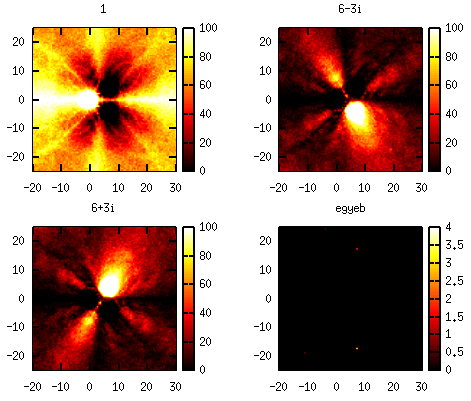
\includegraphics[scale=0.65]{Konv2.png}
					\caption{\ref{lst:konvabra} listázás eredménye. Adott gyökhöz tartozó ábra minél világosabb egy adott pontban, annál többször konvergál a véletlen iteráció hozzá. Míg a véletlenül kiválasztott kezdőpontunknál véletlenül 1 valószínűséggel konvergált egy adott gyökhöz a módszer, itt látható, hogy ez nincs mindig így.} \label{fig:konv_el}
				\end{figure}
				
				Bár az eredmény a \ref{fig:konv_el} ábrán érdekes szabályosságot mutat, sok mindent erről a részletesebb ábráról sem tudunk megállapítani. Feltünő viszont, hogy a valós gyökhöz mennyivel többször konvergál a módszer.
				
				Amennyiben a \ref{lst:iter} program által generált adatokat nem kirajzoljuk, hanem egy változóba mentjük, úgy további elemzéseket tudunk végrehajtani. Legyen \ref{lst:piter} listázás  eredménye a \texttt{zs} változóba mentve a következőképpen. \texttt{zs} 6 db mátrixot tartalmaz. Az első mátrix (\texttt{zs(:,:,1)}) a Newton-módszerhez szükséges lépések száma, a második a Newton-módszerhez szükséges lépések száma $p/p'$ egyenleten, a harmadik a véletlen iterációhoz szükséges lépések számának minimuma, negyedik az átlaga, ötödik a maximuma.

				Vizsgáljuk meg lehet-e a véletlen iteráció gyorsabb, mint valamelyik egyenleten alkalmazott Newton-módszer.
				\begin{lstlisting}[caption=Bemenet,label=lst:min]
t=min(zs(:,:,1),zs(:,:,2))>zs(:,:,3);
[x y]=meshgrid(linspace(-20,30,100),linspace(-25,25,100));
figure
pcolor(x,y,double(t))
axis equal tight;
colorbar;
colormap hot;
shading flat;
sum(sum(t))/10000
				\end{lstlisting}
				Ezzel kirajzoltuk, hogy hol, és megszámoltuk, hogy milyen arányban lett a véletlen iteráció gyorsabb mindkét eljárásnál. 
				\begin{lstlisting}[caption= Eredm\'eny]
ans =  0.32470
				\end{lstlisting}
				Ez egész jó eredmény, de figyelembe kell venni, hogy minden pontban 100 futtatásnak a minimumát vettük, vagyis nem azt jelenti, hogy 1/3 az esélyünk arra, hogy gyorsabb lesz a módszerünk az adott síkrészen.
				
				\begin{figure}[ht]
					\centering
					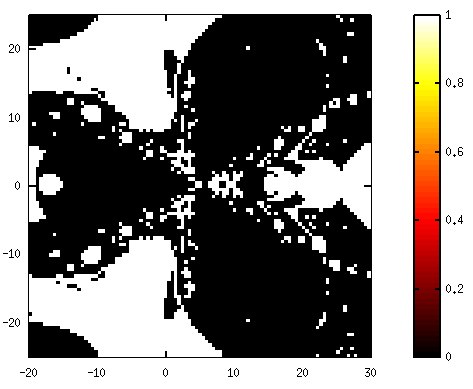
\includegraphics[scale=0.35]{min.png}
					\caption{\ref{lst:min} listázás eredménye. A fehér mezőkben található komplex számokból indított véletlen iterációk gyorsabbak lettek mint külön-külön alkalmazva az első és második iterációs lépéseket. Ami nem egyezik meg a \ref{k11} ábra alapján várt eredménnyel. Ezek a pontok a adott síkrészen a $100\cdot100$ pontnak a $32,\!47\%$-át teszik ki.}
				\end{figure}

				A \ref{lst:first} listázás eredményéből úgy tűnik, hogy a véletlen iteráció szükséges lépésszámának az átlaga a gyorsabb iterációs lépés szükséges lépésszámához van közelebb. Ezt az elmentett adatokból meg tudjuk vizsgálni.
				\begin{lstlisting}[caption=Bemenet]
t=abs(min(zs(:,:,1),zs(:,:,2))-zs(:,:,4))<abs(max(zs(:,:,1),zs(:,:,2))-zs(:,:,4));
sum(sum(t))/10000
				\end{lstlisting}
				Az 1. sorban létrehozok egy olyan mátrixot melynek elemei logikai változók: igaz, ha a gyorsabb iterációs lépéshez, hamis ha a lassabb iterációs lépéshez van közel az átlag. a 2. sorban kiszámoljuk ennek valószínűségét.
				\begin{lstlisting}[caption=Eredm\'eny]
0.10780
				\end{lstlisting}
				Eszerint a hivatkozott eredmény félrevezető volt. Vizsgáljuk meg, hogy mikor fordul elő, hogy a lassabb iterációs lépéshez közelít az átlag.
		        \begin{lstlisting}[caption=Bemenet,label=lst:feltP]		
A=abs(min(zs(:,:,1),zs(:,:,2))-zs(:,:,4))<abs(max(zs(:,:,1),zs(:,:,2))-zs(:,:,4));
t=max(zs(:,:,1),zs(:,:,2))-min(zs(:,:,1),zs(:,:,2));
x=1:23;
y=zeros(1,23);
for i=x
    B=t>i;
    pAB=sum(sum(A & B))/10000;
    pB=sum(sum(B))/10000;
    y(i)=pAB/pB;
end
plot(x,y)
                \end{lstlisting}
                Megnéztük, hogy mi a valószínűsége annak, hogy a minimumtól való távolság kisebb mint a maximumtól való távolság, feltéve, hogy a minimum és a maximum távolsága nagyobb mint $x$, ahol $x\in [1,23]$ egész szám. Ezt minden $x$-re kirajzoltuk.
                
                \begin{figure}[ht]
					\centering
					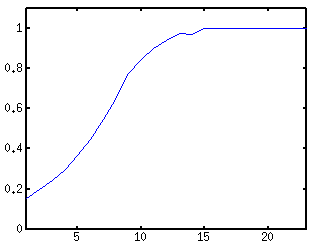
\includegraphics[scale=0.7]{feltP.png}
					\caption{\ref{lst:feltP} listázás eredménye, mely azt ábrázolja, hogy adott $x$-re mekkora a feltételes valószínűsége, hogyha az első és második iterációs lépéshez szükséges lépészszámok különbsége nagyobb mint $x$, akkor a véletlen iterációhoz szükséges lépésszámok átlaga a gyorsabb iterációs lépésnek a szükséges lépésszámához van közel. Az ábra szerint $x=15$-től ennek feltételes valószínűsége 1.}
				\end{figure}
				
				Eszerint ez a tendencia a gyöktől távol vagy megváltozik, vagy az először véletlenül kiválasztott pontunk éppen olyan pont volt, ahol a két iterációs lépéshez szükséges lépésszám között elég nagy volt a különbség. Valószínűnek tartom, hogy mindkettő igaz, és a megváltozott tendencia nem más, mint a gyöktől távol a két iterációs lépéshez szükséges lépésszám egymástól való eltávolodása, ami egyébként intuitív logikus, hiszen két különböző iterációs lépés miért lenne mindenhonnan nagyjából ugyanolyan gyors. 



			\subsection{Érdekes esetek}
				\todoor{2013.05.14: Ezt a részt most kezdtem el, sajnos még nem értek véget a futtatások.}Érdekes esetnek tartom amikor a két iterációs lépés közül legalább az egyik nem konvergál semelyik gyökhöz. Vizsgáljuk meg a véletlen iteráció ilyen esetekben, hogyan viselkedik.

				Vegyük azt a két példát amit a 2. fejezet végén a komplex esetnél bemutattam, és nézzük meg az adott tartományokon milyen hányszor és milyen gyorsan konvergál.
               	\begin{lstlisting}[caption=Bemenet,label=erdekes1]
IteracioAbraKomplex(poly([1,-0.5-0.33i,-0.5+0.33i]),-0.2-0.2i,0.2+0.2i,100,100,3)
                \end{lstlisting}
                A $f(x) = (x-1)\cdot (x+0,\!5+0,\!33i) \cdot (x+0,\!5-0,\!33i)$ polinomot az egyszerűség kedvéért ugyanazon a halmazon ábrázoltam mint \ref{img:div} ábrán. 
                
                \begin{figure}[htp]
					\centering
					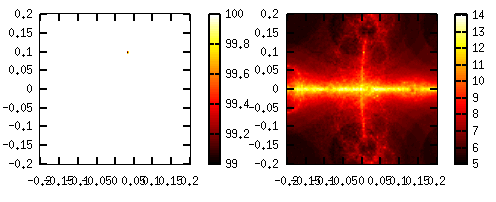
\includegraphics[scale=0.7]{erdekes.png}
					\caption{\ref{erdekes1} listázás eredménye, melyről látható, hogy a véletlen iteráció olyan helyről is konvergálhat, ahol az első iterációs lépés nem.}
				\end{figure}
                
                \begin{lstlisting}[caption=Bemenet,label=erdekes2]
IteracioAbraKomplex(poly([1,3,5+j]),0,5+5j,100,1,2)
IteracioAbraKomplex(poly([1,3,5+j]),0,5+5j,100,100,3)
				\end{lstlisting}
                
                \begin{figure}[hpp]
					\centering
					\subfigure[Az második iterációs lépéssel]{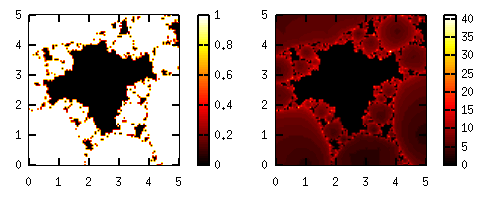
\includegraphics[scale=0.7]{erdekes2.png}}
					\subfigure[A véletlen iterációval]{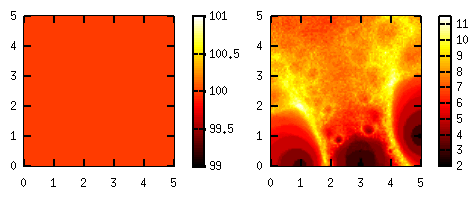
\includegraphics[scale=0.7]{erdekes3.png}}
			        \caption{\ref{erdekes2} listázás eredménye, melyről látható, hogy a véletlen iteráció olyan helyről is konvergálhat, ahol a második iterációs lépés nem.}
				\end{figure}
                
                

			\subsection{Ellenpélda}
                Az előzőekben bemutattunk egy példát amin a véletlen iteráció viszonylag jól viselkedett, azonban könnyen találhatunk olyan példát ahol a módszer meglehetősen rosszul viselkedik. A következőkben egy ilyet vizsgálunk.
                
                Vegyük az $x^3-1$ polinomot melyet korábban már ábrázoltam a \ref{k10} ábrán. Ennek gyökei a következők: $1, -1/2+i\sqrt{3}/2, -1/2-i\sqrt{3}/2$. Ez a gyökök elhelyezkedését nézve hasonló az előzőekben vizsgált polinomhoz, azonban itt a gyökök a komplex síkon egy szabályos háromszög csúcsain helyezkednek el. E hasonlóság miatt érdekes összehasonlítani a két példát.
                \begin{lstlisting}[caption=Bemenet,label=str:ellen1]
p=[1 0 0 -1];
IteracioAbraKomplex(p,-5-5i,5+5i,100,1,1)
IteracioAbraKomplex(p,-5-5i,5+5i,100,1,2)
                \end{lstlisting}
                Lefuttatjuk a már ismert programunkat amely kirajzolja a szükséges iterációs lépések számát az adott módszerekhez a $\{a+bi:a,b\in[-5,5]\}$ síkrészen.
                
                \begin{figure}[ht]
					\centering
					\subfigure[Az első iterációs lépéssel]{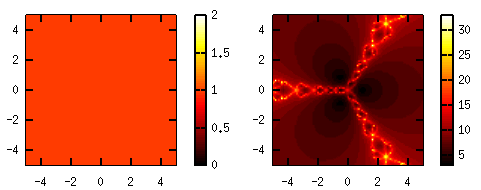
\includegraphics[scale=0.7]{ellenpelda2.png}}
					\subfigure[A második iterációs lépéssel]{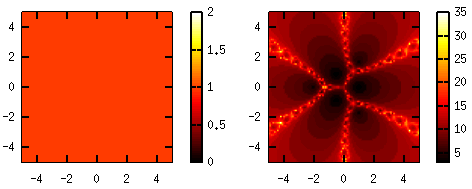
\includegraphics[scale=0.7]{ellenpelda1.png}}
			        \caption{\ref{str:ellen1} listázás eredménye}
				\end{figure}
				
                Láthatjuk, hogy a két iterációs lépés külön-külön minden vizsgált kezdőpontból konvergens volt, azonban a véletlen iterációnál ez megváltozik.
                \begin{lstlisting}[caption=Bemenet,label=lst:ellen2]
KonvergenciaAbraKomplex(p,-5-5i,5+5i,100,100,3)
                \end{lstlisting}
                Kirajzoljuk a gyökökhöz tartozó vonzási tartományok véletlen iterációhoz tartozó megfelelőjét.
                
                \begin{figure}[ht]
					\centering
					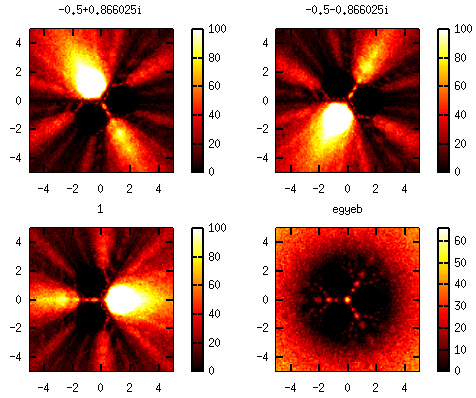
\includegraphics[scale=0.6]{veletlen.png}
					\caption{\ref{lst:ellen2} listázás eredménye, mely azt ábrázolja, hogy melyik komplex számból melyik gyökhöz hányszor konvergált a véletlen iteráció. Látható a különbség \ref{fig:konv_el} ábrától. Míg a jelenlegi ábrán minden gyökhöz azonos ábra tartozik egy megfelelő 120 fokos forgatás erejéig, addig a másik ábrán a valós gyök magához vonzotta azokat az iterációkat amik most az egyéb halmazba estek.}
				\end{figure}

Az eredmény az eddigiek alapján meglepő lehet, hiszen a polinomunkon a véletlen iteráció annak három gyökéhez közeli intervallumon is már rosszabbul viselkedik mint azt elvárnánk, ráadásul egy olyan polinomon, aminek gyökei hasonlóan helyezkedtek el egymáshoz viszonyítva, a módszer meglehetősen jól viselkedett. A különbség az volt, hogy az előző polinomunk gyökei nem egy szabályos háromszögben helyezkedtek el a komplex síkon, míg most igen. Felvetődik tehát a kérdés, hogy vajon a szabályos háromszöggel van-e a baj, és ha igen akkor miért rontja el a módszerünket.

Futtassunk le egy kis programot amely véletlenszerűen generál 3 gyököt az $\{ a+bi : a,b \in [-10,10]\}$ halmazból, és nézzük meg ezeken hogyan viselkedik a módszer. Ehhez szükség van a \ref{lst:iter} program kisebb módosítására: adjuk a $z$ mátrixot visszatérési értékül. A $z$ mátrix tartalmazza, hogy adott pontból hányszor konvergált gyökhöz az iteráció.
                \begin{lstlisting}[caption=Bemenet,label=lst:szabalyos]
k=0;
for i=1:100
    gyok=(rand(6,1)*(20))-10;
    x=IteracioAbraKomplex(poly([gyok(1)+gyok(2)*j,gyok(3)+gyok(4)*j,gyok(5)+gyok(6)*j]),-100-100j,100+100j,10,10,3);
    if sum(sum(x))==10^3
        k=k+1;
    end
end
k/100
                \end{lstlisting}
A program $6$ valós számot generál $-10$ és $10$ között, amiből létrehoz $3$ komplex számot, ezekből létrehoz egy polinomot, és lefuttatja rá a \ref{lst:iter} programot, a fent említett módosítással. A program a $\{a+bi:a,b\in[-100,100]\}$ halmazon fut, mivel az ábrán az figyelhető meg, hogyha a véletlen iteráció rossz, akkor a gyököktől távolabb kezd el romlani. $10\cdot 10$ pontból indítjuk a véletlen iterációt, amit $10$-szer megismétel adott polinomra, majd az egészet még $100$-szor, vagyis 100 ilyen polinomra.
                \begin{lstlisting}[caption=Eredm\'eny]
ans =  0.98000
                \end{lstlisting}
Vagyis a polinomok 98\%-án minden esetben annyiszor érte el a gyököt a módszer, ahányszor futtattuk. Most generáljunk olyan polinomokat amiknek a gyökei szabályos sokszögként helyezkednek el.
                \begin{lstlisting}[caption=Bemenet]
k=0;
for i=1:100
    gyok=(rand(4,1)*(20))-10;
    gyok(5:6)=[cos(pi/3),-sin(pi/3);sin(pi/3),cos(pi/3)]*[gyok(3)-gyok(1);gyok(4)-gyok(2)]+[gyok(1);gyok(2)];
    x=IteracioAbraKomplex(poly([gyok(1)+gyok(2)*j,gyok(3)+gyok(4)*j,gyok(5)+gyok(6)*j]),-100-100j,100+100j,10,10,3);
    if sum(sum(x))==10^3
        k=k+1;
    end
end
k/100
                \end{lstlisting}
A program $4$ valós számot generál $-10$ és $10$ között, amiből létrehoz két komplex számot. Ezeket vektorként alkalmazva egy forgásmátrix segítségével létrehozzuk a harmadik gyököt, majd az előzőekben ismertetett módon folytatjuk az eljárást.
                \begin{lstlisting}[caption=Eredm\'eny]
ans = 0
                \end{lstlisting}
Látható, ha céltudatosan olyan polinomot generálunk amelynek gyökei a komplex síkon szabályos háromszögként helyezkednek el, akkor ez az eredmény nemcsak drasztikusan lecsökken, de egyenesen egy ilyen típusú polinomra sem volt konvergens minden esetben amikor futtattuk rajta a módszert. Persze ez egy erős feltétel, de láthatjuk, hogy a véletlenszerűen elhelyezkedő gyököknél ekkor is magas volt a százalék. Ha a 6. sort átírjuk a következőre: 
\begin{lstlisting}[firstnumber=6]
if sum(sum(x))>=10^3*0.5
\end{lstlisting}
ami azt jelenti, hogy egy adott polinomnál csak azt szeretnénk, hogy a rajta indított véletlen iterációk fele legyen konvergens (az adott feltételek mellett), akkor az eredmény $0,\!12$-re emelkedik.

Érdemes megvizsgálni negyedfokú polinomok körében is ezt a viselkedést. Helyettesítsük \ref{lst:szabalyos} listázás 3-4. sorát a következővel:
\begin{lstlisting}[firstnumber=3]
gyok=(rand(8,1)*(20))-10;
x=IteracioAbraKomplex(poly([gyok(1)+gyok(2)*j,gyok(3)+gyok(4)*j,gyok(5)+gyok(6)*j,gyok(7)+gyok(8)*j]),-100-100j,100+100j,10,10,3);
\end{lstlisting}
amivel 4 darab komplex gyökkel rendelkező polinomokra futtatjuk a módszert.
                \begin{lstlisting}[caption=Eredm\'eny]
ans =  0.97000
                \end{lstlisting}
Hasonlóan jó eredményt kapunk. Most generáljunk szabályos négyszögben elhelyezkedő gyököket.
\begin{lstlisting}[caption=Bemenet]
k=0;
for i=1:100
    gyok=(rand(4,1)*(20))-10;
    elt=[0,-1;1,0]*[gyok(3)-gyok(1);gyok(4)-gyok(2)];
    gyok(5:6)=elt+[gyok(1);gyok(2)];
    gyok(7:8)=elt+[gyok(3);gyok(4)];
    x=IteracioAbraKomplex(poly([gyok(1)+gyok(2)*j,gyok(3)+gyok(4)*j,gyok(5)+gyok(6)*j,gyok(7)+gyok(8)*j]),-100-100j,100+100j,10,10,3);
    if sum(sum(x))==10^3
        k=k+1;
    end
end
k/100
\end{lstlisting}
Mint az előbb, egy eltolásvektort hozunk létre, a derékszögű forgásmátrix segítségével, amivel létrehozunk 2 pontból 4 szabályos négyszögben elhelyezkedőt.
                \begin{lstlisting}[caption=Eredm\'eny]
ans =  0
                \end{lstlisting}
Az eredmény megfelel a harmadfokú polinomokon tapasztalttal. Ha itt is módosítjuk, hogy adott polinomra csak az indított iterációk 50\%-a legyen konvergens akkor az eredmény $0,\!64$-re emelkedik. Ez nagyobb emelkedés mint amit harmadfokú esetben láthattunk.

Ezáltal úgy sejtjük, hogy ha a egy polinom gyökei szabályos sokszögként helyezkednek el a komplex síkon a módszer, a gyököktől megfelelően távolról indulva, pozitív valószínűséggel divergál.

\chapter{Összefoglalás}
\todoor{2013.05.14: megírtam az összefoglalást}
Dolgozatom során egy olyan iterációs módszer vizsgálatával foglalkoztam, amely véletlenszerűen lép két iterációs lépés segítségével. A két iterációs lépés igazából nem más, mint az egyenletünkön, és annak egy olyan módosításán végzett iterációs módszer, amelynek gyökei megegyeznek az eredeti egyenletünkével. Ennek a koncepciónak azt a speciális esetét vizsgáltam amikor a két egyenleten a Newton-módszert hajtom végre. Ehhez szükség volt a Newton-módszer alapos bemutatására és megismerésére. 

A második fejezet során láthattuk, hogy a Newton-módszer milyen egyszerű koncepción alapszik, és ha bizonyos feltételek teljesülnek és a módszer konvergens, akkor a módszer másodrendben tart a gyökhöz. Megállapítottuk, milyen feltételek szükségesek a konvergenciához, és azt is, hogy bizonyos feltételekkel monoton konvergenciát tudunk biztosítani. Megvizsgáltuk, a komplex gyökökkel rendelkező egyenletekre mi a geometriai meggondolás, melyből kiderült, hogy a Newton-módszer egy gradiens módszer $|f|$ abszolút érték függvényre nézve. A komplex síkon minden gyökhöz tartozik egy vonzási tartomány, melyek másodfokú polinomok esetén két félsíkot, magasabb fokú polinomok és egyéb komplex differenciálható függvények esetén különböző fraktálokat határoznak meg.

A következőkben a módszerünket polinomokra specializáltuk, amelyeknél a módosított egyenletet úgy állítottuk elő, hogy az eredeti polinomot leosztottuk egy másikkal, amire a saját deriváltját választottuk. Megmutattuk, hogy egy-két plusz feltétellel a második iterációs lépés is másodrendben konvergens, és még a többszörös gyök sem biztos, hogy megakadályozza a konvergenciát. Ezután a módszer elemzéséhez általam írt számítógépes programokat használtunk fel. A következő fontosabb eredményeket tapasztaltuk: A módszer gyorsasága átlagosan a két iterációs lépés gyorsasága között mozog, azonban van esélyünk arra is, hogy gyorsabb, és arra is, hogy lassabb legyen mindkét iterációs lépésnél. Ha a két iterációs lépéshez szükséges lépésszám között nagy a különbség, akkor a véletlen iterációhoz szükséges átlagos lépésszáma a gyorsabb iterációs lépésnek a szükséges lépésszámához van közelebb, ami kedvező hiszen semmi sem garantálja a két iterációs lépés gyorsaságának a hasonlóságát. Azonban a módszer valamilyen oknál fogva rosszul viselkedik olyan polinomokon amelyeknek a gyökei szabályos sokszögként helyezkednek el a komplex síkon.




\begin{appendices}
	\chapter{A dolgozatban használt programok bemutatása} \label{Appendix}
		A dolgozatban felhasznált programok GNU Octave nyelven íródtak ami egy ingyenes MATLAB klón, ezáltal a következő programok jó eséllyel lefutnak MATLAB-ban, viszont előfordulhatnak kisebb kompatibilitási hibák. Ezeket azonban általában könnyen és hamar ki lehet küszöbölni. További probléma, hogy az említett programnyelvek lassan kezelik a \texttt{for} ciklusokat, helyette a műveletek vektorokkal való megoldását javasolják. Az alábbi programok több egymásba ágyazott \texttt{for} ciklust használnak, ezáltal meglehetősen lassúak lehetnek.
		
		\section{A felhasznált módszerek megvalósítása} \label{Newton}
			\begin{lstlisting}[caption=Newton.m]
function [gyok it]=Newton(p,x0,seq=0,m=1,h=0.001,maxit=100,prob=0.5)
    x(1)=x0;                                                        
    pd=polyder(p);                                                  
    pdd=polyder(pd);                                                
    if m==3                                                         
        r=1;                                                        
    else                                                            
        r=0;                                                        
    end                                                             
    for i=2:(maxit+1)                                               
        px=polyval(p,x(i-1));                                       
        pdx=polyval(pd,x(i-1));                                     
        if r==1                                                     
            if(rand>prob)                                           
                m=1;                                                
            else                                                    
                m=2;                                                
            end                                                     
        end                                                         
                                                                    
        if m==1                                                     
            if pdx==0                                               
                i=i-1;                                              
                break;                                              
            end                                                     
            x(i)=x(i-1)-px/pdx;                                     
        elseif m==2                                                 
            pddx=polyval(pdd,x(i-1));                               
            if pdx^2-pddx*px==0                                     
                i=i-1;                                              
                break;                                              
            end                                                     
            x(i)=x(i-1)-(px*pdx)/(pdx^2-pddx*px);                   
        end                                                         
                                                                    
        if ( abs(x(i)-x(i-1)) < h*abs(x(i)) )                       
            break;                                                  
        end                                                         
    end                                                             
    it=i-1;                                                         
    if seq==0                                                       
        gyok=x(i);                                                  
    else                                                            
        gyok=x;                                                     
    end                                                             
			\end{lstlisting}
			A listázott program végzi minden felhasznált programban a Newton-módszert egy adott polinomra és annak módosított egyenletére, és a módosított módszert is.
			        
            A bemeneti változók:
			\begin{enumerate}
				\item[p:] Adott polinom együtthatói vektorként, ahol a legnagyobb kitevő együtthatója az első elem, és utána a sorban a többi.
				\item[x0:] Kezdőpont
				\item[seq:] Ha 1, akkor a gyok visszatérési típusa a lépések tömbje, ha 0 akkor csak az utolsó lépés
				\item[m:] Módszer sorszáma. 1: Newton-módszer $p$-re, 2: Newton-módszer $p/p'$-re, 3: Véletlen iteráció
				\item[h:] A leállási feltételhez használt hibahatár
				\item[maxit:] Maximum megengedett iteráció
				\item[prob:] A véletlen iterációnál a módosított egyenletre történő Newton-módszer valószínűsége
			\end{enumerate}
			A felsoroltakból csak az első két paramétert kötelező megadni, ez esetben alapbeállításokkal végzi a módszert.

		\section{Konvergencia szemléltetése} \label{Konvergencia}
			\begin{lstlisting}[caption=IteracioAbraKomplex.m,escapeinside={@}{@},label=lst:iter]
function IteracioAbraKomplex(p,a,b,f,ism,m=3,h=0.001)                               
    [x y]=meshgrid(linspace(real(a),real(b),f),linspace(imag(a),imag(b),f));
    r=roots(p);                                                             
    n=length(r)+1;                                                          
    z=zeros(f,f);                                                           
    zs=zeros(f,f);                                                          
    it_temp=zeros(ism);                                                     
    for k=1:f                                                               
        for l=1:f                                                           
            temp=0;                                                         
            for i=1:ism                                                     
                [gyok,it]=Newton(p,x(k,l)+y(k,l)*j,0,m,h,60);               
                [MINE MINH]=min(abs(r-gyok));                               
                if MINE<h                                                   
                    z(k,l)=z(k,l)+1;                                        
                    temp=temp+1;                                            
                    it_temp(temp)=it;                                       
                end                                                         
            end                                                             
            if temp!=0                                                      
@\label{lst:mean}@                zs(k,l)=mean(it_temp(1:temp)); 
            else                                                            
                zs(k,l)=0;                                                  
            end                                                             
        end                                                                 
    end                                                            
    figure                                                                  
    subplot(1,2,1)                                                          
    pcolor(x,y,z)                                                           
    colorbar;                                                               
    colormap hot;                                                           
    shading interp;                                                         
    axis equal tight;                                                       
    subplot(1,2,2)                                                          
    pcolor(x,y,zs)                                                          
    colorbar;                                                               
    colormap hot;                                                           
    shading interp;                                                         
    axis equal tight;
			\end{lstlisting}
			A listázott program elvégzi az adott iterációs eljárást egy a komplex síkról vett téglalapon megadott sűrűséggel és ismétlésszámmal, majd két ábrát generál belőle. Az első ábra szemlélteti, hogy az ismétlésszámból mennyi iteráció ért célt valamelyik gyöknél. A második ábra az iterációhoz szükséges átlagos lépésszámot szemlélteti. Az ábrákon a világosabb szín jelöli a nagyobb számot.
			\begin{enumerate}
				\item[p:] Adott polinom együtthatói vektorként, ahol a legnagyobb kitevő együtthatója az első elem, és utána a sorban a többi.
				\item[a:] A kívánt téglalap bal alsó sarkában elhelyezkedő komplex szám
				\item[b:] A kívánt téglalap jobb felső sarkában elhelyezkedő komplex szám
				\item[f:] $f^2$ kezdőpontra osztjuk a téglalapot
				\item[ism:] Adott kezdőpontra hányszor ismételjük meg az iterációs módszert
				\item[m:] Módszer sorszáma. 1: Newton-módszer $p$-re, 2: Newton-módszer $p/p'$-re, 3: Véletlen iteráció
				\item[h:] A leállási feltételhez használt hibahatár
			\end{enumerate}
			\begin{Megj}\label{app:megj}
				Az generált ábrából egy kevés módosítással más információt is kinyerhetünk. A \ref{lst:mean}. sorban a \texttt{mean} függvényt helyettesíthetjük különböző statisztikai függvényekkel mint a \texttt{min}, \texttt{max}, vagy az \texttt{std} függvénnyel mely szórást számol.
			\end{Megj} 
			\begin{lstlisting}[caption=KonvergenciaAbraKomplex.m]
function KonvergenciaAbraKomplex(p,a,b,f,ism,m=3,h=0.001)
    [x y]=meshgrid(linspace(real(a),real(b),f),linspace(imag(a),imag(b),f));
    r=unique(roots(p));
    n=length(r)+1;
    z=zeros(f,f,n);
    for i=1:ism
        for k=1:f
            for l=1:f
                [gyok,it]=Newton(p,x(k,l)+y(k,l)*j,0,m,h,120);
                [MINE MINH]=min(abs(r-gyok));
                if MINE<h
                    z(k,l,MINH)=z(k,l,MINH)+1;
                else
                    z(k,l,n)=z(k,l,n)+1;
                end
            end
        end
    end

    figure
    for j=1:n
        subplot(ceil(n/2),2,j)
        pcolor(x,y,z(:,:,j))
        colorbar;
        colormap hot;
        shading interp;
        axis equal tight;
        if j!=n
            title(num2str(r(j)));
        else
            title('egyeb');
        end
    end
			\end{lstlisting}
			A listázott program elvégzi az adott iterációs eljárást egy a komplex síkról vett téglalapon megadott sűrűséggel és ismétlésszámmal, majd gyökszám plusz egy ábrát generál belőle. Mindegyik gyökhöz tartozott ábra azt szemlélteti hányszor konvergált hozzá a módszer. Az utolsó ábra szemlélteti azokat az iterációkat amik nem értek el egy gyököt.

			A metódus paraméterei megegyeznek \ref{lst:iter} listázás paramétereivel.
\end{appendices}

% irodalomjegyzék
	\begin{thebibliography}{99}
    	\bibitem{jr} E. T. Whittaker, G. Robinson, ``The Newton-Raphson Method'' \emph{The Calculus of Observations: A Treatise on Numerical Mathematics, 4th ed.}, New York: Dover, pp. 84-87, 1967. 
		\bibitem{aa} Faragó István, \emph{Alkalmazott analízis 1}, előadás jegyzet 2012.
        \bibitem{na} Faragó István, Horváth Róbert, ``Nemlineáris egyenletek és egyenletrendszerek megoldása'' \emph{Numerikus módszerek}, Typotex 2011.
        \bibitem{Yau98} Lily Yau, Adi Ben-Israel ``The Newton and Halley Methods for Complex Roots'', \emph{The American Mathematical Monthly} Vol. 105, No. 9, November 1998. % http://folk.uib.no/ssu029/Pdf_file/Yau98.pdf
		\bibitem{calculus} P.D. Straffin, C.C.T. Benson, \emph{Calculus Problems for a New Century}, Mathematical Association of America 1993.
	\bibitem{div} William J. Gilbert, ``Generalizations of Newton's method'', \emph{Fractals} Vol. 9, No. 3,  Szeptember 2001.

        
	\end{thebibliography}
\end{document}
